\chapter{Cálculos de Aerodinâmica e Desempenho}

As análises conduzidas neste capítulo utilizam os pesos definidos na Tabela~\ref{tab:cg_entradas}, selecionados conforme a condição operacional de cada fase de voo.

\section{Cálculo da Polar de Arrasto}

Nesta seção, determina-se a curva $C_D \times C_L$ da aeronave regional de projeto, que serve como base fundamental para mapear o envelope aerodinâmico e subsidiar todos os cálculos subsequentes de desempenho em missão. A polar de arrasto global é modelada analiticamente pela equação quadrática:
\begin{equation}
    C_D = C_{D_0} + B \cdot C_L + A \cdot C_L^2
\end{equation}

Para uma plataforma de transporte comercial deste porte, o arrasto parasita total engloba mais do que o atrito superficial e a pressão dos componentes principais. Uma parcela significativa do $C_{D_0}$ provém de arrastos de miscelânea e penalidades aerodinâmicas causadas por:
\begin{itemize}
    \item \textbf{Interferência:} O gradiente de pressão adverso gerado na junção física de grandes componentes (como a raiz da asa alta com o topo da fuselagem ou a cauda convencional);
    \item \textbf{Leaks e Gaps:} Frestas em superfícies de comando de grande extensão (ailerons, flaps) e portas de inspeção ou serviço;
    \item \textbf{Sistemas de Refrigeração e Admissão:} Perda de quantidade de movimento do ar captado para os motores e trocadores de calor.
\end{itemize}

Uma estimativa refinada do coeficiente de arrasto parasita total ($C_{D_0}$) exige ensaios em túnel de vento ou análises de CFD de alta fidelidade. Para o escopo desta etapa de projeto, ele será estimado de forma analítica e empírica segundo o procedimento consolidado em \cite{Pullin}.

Segue a apresentação das metodologias e valores calculados para as parcelas que compõem o balanço de $C_{D_0}$ final da aeronave.

\section{Estimativa do Arrasto Parasita da Fuselagem ($C_{D_{0f}}$)}

A equação governante utilizada para este modelo é expressa por:
\begin{equation}
    C_{D_{0f}} = C_{D_{0A}} + C_{D_{0B}} + C_{D_{0C}} + \Delta C_{D_{\Lambda F}} + \Delta C_{D_{0CAB}}
\end{equation}

Onde os coeficientes de arrasto viscoso para as seções dianteira (A), central (B) e traseira (C) são definidos pelas relações:
\begin{equation}
    C_{D_{0A}} = \frac{C_f \cdot F \cdot S_M^A}{S}
\end{equation}
\begin{equation}
    C_{D_{0B}} = \frac{C_f \cdot F \cdot S_M^B}{S}
\end{equation}
\begin{equation}
    C_{D_{0C}} = \frac{C_f \cdot F \cdot S_M^C}{S}
\end{equation}

Sendo:
\begin{itemize}
    \item $C_{D_{0A}}$, $C_{D_{0B}}$, $C_{D_{0C}}$: Coeficientes de arrasto das respectivas seções;
    \item $C_f$: Coeficiente de atrito médio da superfície;
    \item $F$: Fator de forma da fuselagem;
    \item $S_M^A$, $S_M^B$, $S_M^C$: Áreas molhadas das seções A, B e C;
    \item $S$: Área da asa (referência).
\end{itemize}

\subsection{Coeficiente de atrito médio da superfície ($C_f$)}

O procedimento baseou-se na relação entre o comprimento característico do corpo e a rugosidade equivalente do material. Utilizando o software SolidWorks, mensurou-se o comprimento total da fuselagem ($l_f$). O parâmetro de rugosidade ($k$) foi estimado com base na literatura para uma superfície com acabamento de "pintura cuidadosa" (smooth paint). 

A partir da razão de esbeltez aerodinâmica ($l_f / k$), obteve-se o coeficiente de atrito para as diferentes fases de voo consultando-se os ábacos e tabelas de atrito para placas planas.
%disponibilizados na seção de Anexos deste documento (ver Figuras \ref{fig:rugosidade} e \ref{fig:diagrama_cf}).

Os parâmetros geométricos e os coeficientes de atrito obtidos para as condições de Cruzeiro, Decolagem e Pouso estão consolidados nas Tabelas \ref{tab:parametros_rugosidade} e \ref{tab:coef_atrito}.

\begin{table}[H]
    \centering
    \caption{Parâmetros geométricos e de rugosidade estimados.}
    \vspace{0.2cm}
    \begin{tabular}{lc}
        \toprule
        \textbf{Parâmetro} & \textbf{Valor} \\
        \midrule
        Comprimento da Fuselagem ($l_f$) [SolidWorks] & 26 m \\
        Rugosidade ($k$) [Pintura Cuidadosa] & 0,0064 m \\
        Razão de Rugosidade ($l_f / k$) & 4062,5 \\
        \bottomrule
    \end{tabular}
    \label{tab:parametros_rugosidade}
\end{table}

\begin{table}[H]
    \centering
    \caption{Coeficientes de atrito médio.}
    \vspace{0.2cm}
    \begin{tabular}{lc}
        \toprule
        \textbf{Condição de Voo} & \textbf{Coeficiente ($C_f$)} \\
        \midrule
        Cruzeiro & 0,0065 \\
        Decolagem & 0,0060 \\
        Pouso & 0,0060 \\
        \bottomrule
    \end{tabular}
    \label{tab:coef_atrito}
\end{table}

\subsection{Fator de Forma e Coeficientes por Seção}

O Fator de Forma ($F$) é um parâmetro adimensional que corrige o arrasto de atrito para englobar os efeitos do gradiente de pressão causados pela espessura finita da fuselagem. A determinação deste fator depende diretamente da geometria da aeronave, especificamente da relação conhecida como Esbeltez Efetiva ($E_e$).

A esbeltez efetiva é calculada considerando apenas as seções de afilamento (nariz e cauda), ignorando a seção central cilíndrica, relacionando o comprimento dessas partes com o diâmetro equivalente máximo do corpo ($D_{eq} = 2,96$ m).

\begin{equation}
    E_e = \frac{l_a + l_c}{D_{eq}}
\end{equation}

Substituindo os valores geométricos obtidos via CAD ($l_a = 3,5$ m e $l_c = 6,5$ m), obteve-se uma esbeltez efetiva de:
\begin{equation}
    E_e = 3,378
\end{equation}

Com este valor, determinou-se o Fator de Forma através da consulta ao gráfico empírico de correlação geométrica, resultando em:
\begin{equation}
    F = 1,33
\end{equation}

De posse do fator de forma ($F$), do coeficiente de atrito ($C_f$) calculado anteriormente e das áreas molhadas de cada seção ($S_a = 26,33 \text{ m}^2$, $S_b = 41,27 \text{ m}^2$ e $S_c = 39,87 \text{ m}^2$), foram calculados os coeficientes de arrasto parasita individuais ($C_{D_{0A}}$, $C_{D_{0B}}$ e $C_{D_{0C}}$).

Os resultados para as três condições de voo analisadas estão consolidados na Tabela \ref{tab:coef_arrasto_fuselagem}.

\begin{table}[H]
    \centering
    \caption{Coeficientes de arrasto parasita por seção da fuselagem.}
    \vspace{0.2cm}
    \begin{tabular}{lccc}
        \toprule
        \textbf{Condição} & \textbf{Seção A ($C_{D_{0A}}$)} & \textbf{Seção B ($C_{D_{0B}}$)} & \textbf{Seção C ($C_{D_{0C}}$)} \\
        \midrule
        Cruzeiro & 0,003 & 0,004 & 0,005 \\
        Decolagem & 0,004 & 0,003 & 0,004 \\
        Pouso & 0,003 & 0,003 & 0,004 \\
        \bottomrule
    \end{tabular}
    \label{tab:coef_arrasto_fuselagem}
\end{table}

\subsection{Acréscimo de Arrasto por Enflechamento Traseiro ($\Delta C_{D_{\Lambda F}}$)}

A geometria da fuselagem traseira, caracterizada por uma curvatura ascendente (\textit{upsweep}), induz uma modificação no campo de pressão local que resulta em uma penalidade aerodinâmica. Este incremento de arrasto é calculado como uma fração do arrasto da seção traseira ($C_{D_{0C}}$), modulada pelo parâmetro de influência $K$:
\begin{equation}
    \Delta C_{D_{\Lambda F}} = \frac{K}{100} \cdot C_{D_{0C}}
\end{equation}

O fator $K$ é dependente direto do ângulo de saída da fuselagem. Utilizando a geometria modelada no software CAD, mensurou-se o ângulo de enflechamento do bordo de fuga:
\begin{equation}
    \Lambda_F = 17,7^{\circ}
\end{equation}

Com este valor, determinou-se o parâmetro $K$ através da consulta ao gráfico de correlação empírica para fuselagens convencionais, obtendo-se:
\begin{equation}
    K = 90
\end{equation}

Aplicando-se este fator aos coeficientes da Seção C calculados anteriormente, obtiveram-se os valores de arrasto adicional para as condições de voo, conforme apresentado na Tabela \ref{tab:arrasto_upsweep}.

\begin{table}[H]
    \centering
    \caption{Acréscimo de Arrasto devido ao Upsweep ($\Delta C_{D_{\Lambda F}}$).}
    \vspace{0.2cm}
    \begin{tabular}{lc}
        \toprule
        \textbf{Condição} & \textbf{Valor} \\
        \midrule
        Cruzeiro & 0,0042 \\
        Decolagem & 0,0039 \\
        Pouso & 0,0039 \\
        \bottomrule
    \end{tabular}
    \label{tab:arrasto_upsweep}
\end{table}

\subsection{Incremento de Arrasto da Cabine ($\Delta C_{D_{0CAB}}$)}

A última parcela considerada para o arrasto isolado da fuselagem quantifica a penalidade aerodinâmica causada pela descontinuidade geométrica e transição do para-brisa na cabine de comando. Esta geometria frontal interrompe o escoamento liso, gerando zonas de sobrepressão localizada cuja magnitude é estimada analiticamente em função da projeção frontal da cabine ($S_{CAB}$) referenciada à nova área da asa do projeto ($S$):
\begin{equation}
    \Delta C_{D_{0CAB}} = 0,07 \cdot \frac{S_{CAB}}{S}
\end{equation}

A área frontal da cabine foi extraída diretamente da projeção frontal do modelo no software CAD, obtendo-se $S_{CAB} = 4,3 \text{ m}^2$. Considerando a área alar de referência $S = 74,1\text{ m}^2$, calculou-se o coeficiente adicional apresentado na Tabela \ref{tab:arrasto_cabine}.

\begin{table}[H]
    \centering
    \caption{Acréscimo de Arrasto devido à Cabine ($\Delta C_{D_{0CAB}}$).}
    \vspace{0.2cm}
    \begin{tabular}{lc}
        \toprule
        \textbf{Condição} & \textbf{Valor} \\
        \midrule
        Cruzeiro & 0,00406 \\
        Decolagem & 0,00406 \\
        Pouso & 0,00406 \\
        \bottomrule
    \end{tabular}
    \label{tab:arrasto_cabine}
\end{table}

\subsection{Consolidação do Arrasto da Fuselagem ($C_{D_{0f}}$)}

Por fim, realizou-se o somatório de todas as componentes aerodinâmicas calculadas anteriormente para determinar o coeficiente de arrasto parasita total da fuselagem. Este valor engloba as parcelas de atrito viscoso das três seções longitudinais ($C_{D_{0A}}$, $C_{D_{0B}}$, $C_{D_{0C}}$) e os incrementos de pressão devidos à geometria do cone de cauda e da cabine.

Aplicando-se os valores na Equação 7.2, obtiveram-se os coeficientes finais para as fases de operação da aeronave, conforme apresentado na Tabela \ref{tab:arrasto_fuselagem_total}.

\begin{table}[H]
    \centering
    \caption{Coeficiente de Arrasto Parasita Total da Fuselagem.}
    \vspace{0.2cm}
    \begin{tabular}{lc}
        \toprule
        \textbf{Condição de Voo} & \textbf{Coeficiente Total ($C_{D_{0f}}$)} \\
        \midrule
        Cruzeiro & 0,026 \\
        Decolagem & 0,025 \\
        Pouso & 0,024 \\
        \bottomrule
    \end{tabular}
    \label{tab:arrasto_fuselagem_total}
\end{table}

Estes valores de $C_{D_{0f}}$ serão integrados ao cálculo do arrasto parasita global da aeronave ($C_{D_0}$), somando-se às contribuições das demais superfícies sustentadoras e componentes externos.

\section{Arrasto do Trem de Pouso ($C_{D_{LG}}$)}

Optou-se pela utilização de um trem de pouso do tipo triciclo retrátil, configuração amplamente empregada em aeronaves comerciais devido às vantagens operacionais e aerodinâmicas associadas. Esse arranjo proporciona maior estabilidade direcional durante o táxi, além de contribuir para operações de pouso e decolagem mais seguras e eficientes. A escolha também se mostra coerente com as aeronaves analisadas no estudo comparativo, que adotam a mesma configuração.

Durante a fase de cruzeiro, assume-se que o trem de pouso permanece completamente recolhido no interior das carenagens e da seção do nariz, com as portas fechadas, de modo que sua influência no arrasto da aeronave pode ser considerada desprezível. Em contrapartida, nas etapas de decolagem e pouso, os componentes ficam expostos ao escoamento, tornando necessária a estimativa do arrasto aerodinâmico associado. Para essa análise, foram utilizados métodos e coeficientes empíricos extraídos da literatura especializada de \textit{Fluid-Dynamic Drag} \cite{Hoerner}.

\subsection{Trem de Nariz}
O coeficiente de arrasto da perna do trem de nariz foi determinado utilizando-se ábacos empíricos que correlacionam o coeficiente de arrasto ($C_{D_\pi}$) com a geometria da perna, o arranjo das rodas e a razão de esbeltez da instalação ($e/d$). %A Figura \ref{fig:trem_nariz}, localizada nos Anexos deste documento, apresenta o gráfico clássico utilizado para a extração deste coeficiente direcional.

\subsection{Trem Principal}
Para o trem de pouso principal, a estimativa baseou-se na decomposição dos elementos estruturais (pernas do amortecedor óleo-pneumático, tesouras de torção e conjunto de rodas) que ficam expostos abaixo das carenagens laterais. Utilizou-se como referência os dados empíricos para arranjos sem carenagens integrais (\textit{unfaired}), conforme ilustrado nos ábacos de referência. %(ver Anexos, Figura \ref{fig:trem_principal}).

\subsection{Cálculo Final do Coeficiente ($C_{D_{LG}}$)}
Como o modelo digital (CAD) da aeronave ainda não contempla o detalhamento completo dos conjuntos de trem de pouso, as áreas frontais projetadas ($S_{ref}$) de cada componente foram estimadas estatisticamente. Utilizaram-se como base as dimensões típicas de pneus e pernas de força de aeronaves escolhidas do estudo comparativo.

Com base nos coeficientes extraídos e nas áreas estimadas, calculou-se a contribuição individual aerodinâmica. O coeficiente total referenciado à área de asa do projeto ($S = 74,1 \text{ m}^2$) é dado pela soma das parcelas do trem de nariz e dos dois conjuntos do trem principal. 

A Tabela \ref{tab:trem_pouso} apresenta os valores detalhados e o coeficiente final obtido.

\begin{table}[H]
    \centering
    \caption{Memória de Cálculo Preliminar do Arrasto do Trem de Pouso.}
    \vspace{0.2cm}
    \begin{tabular}{lc}
        \toprule
        \textbf{Parâmetro / Componente} & \textbf{Valor} \\
        \midrule
        \textbf{Áreas Frontais Estimadas ($m^2$)} & \\
        Área Frontal do Trem de Nariz & 0,165 \\ 
        Área Frontal do Trem Principal & 0,280 \\ 
        \midrule
        \textbf{Coeficientes Parciais (Referência Asa $S = 74,1 m^2$)} & \\
        $C_D$ Trem de Nariz & 0,000850 \\ 
        $C_D$ Trem Principal & 0,002920 \\ 
        \midrule
        \textbf{Coeficiente Total em Configuração Suja ($C_{D_{LG}}$)} & \textbf{0,003770} \\ 
        \bottomrule
    \end{tabular}
    \label{tab:trem_pouso}
\end{table}

\section{Arrastos Adicionais e de Interferência}

Para consolidar o coeficiente de arrasto parasita total em sustentação nula, computam-se as penalidades aerodinâmicas remanescentes que operam de forma isolada na miscelânea do grupo motopropulsor ou nas interseções críticas das superfícies aerodinâmicas com a fuselagem cilíndrica.

\subsection{Arrasto de Acoplamento Asa-Fuselagem}
A interseção de uma asa alta com o contorno superior da fuselagem modifica localmente o campo de velocidade do escoamento potencial, gerando vórtices de junção secundários. Como prática recomendada na literatura preliminar para mitigar e quantificar essa interferência, adicionou-se uma penalidade percentual fixa sobre o coeficiente total já mapeado para o corpo da fuselagem isolado. Adotando-se um fator de interferência de 5\% sobre o $C_{D_{0f}}$ calculado anteriormente, obteve-se o incremento apresentado na Tabela \ref{tab:interferencia_asa_fuselagem}.

\begin{table}[H]
    \centering
    \caption{Arrasto de Interferência Asa-Fuselagem.}
    \vspace{0.2cm}
    \begin{tabular}{lc}
        \toprule
        \textbf{Condição} & \textbf{Incremento ($C_D$)} \\
        \midrule
        Cruzeiro & 0,001 \\
        Decolagem & 0,001 \\
        Pouso & 0,001 \\
        \bottomrule
    \end{tabular}
    \label{tab:interferencia_asa_fuselagem}
\end{table}

\subsection{Arrasto Combinado Empenagens-Fuselagem ($\Delta C_{D_{ef}}$)}
De forma análoga, a união das superfícies da empenagem horizontal e vertical montadas na cauda convencional introduz cantos vivos que geram pequenos descolamentos localizados no cone de cauda. Este coeficiente de interferência nas raízes dos estabilizadores foi calculado analiticamente através da seguinte correlação geométrica clássica:
\begin{equation}
    \Delta C_{D_{ef}} = n_1 \left( 0,8 \left( \frac{t}{c} \right)^3 - 0,0005 \right) \frac{C_i^2}{S}
\end{equation}

Onde:
\begin{itemize}
    \item $n_1 = 2$: Número de cantos vivos na junção estrutural;
    \item $t/c = 0,120$: Espessura relativa do perfil aerodinâmico na raiz da empenagem;
    \item $C_i = 2,47$ m: Corda da empenagem na estação de interseção;
    \item $S$: Área alar de referência da asa.
\end{itemize}

O cálculo resultou em um coeficiente de interferência praticamente desprezível, porém contabilizado:
\begin{equation}
    \Delta C_{D_{ef}} = 0,00007
\end{equation}

\subsection{Arrasto de Hélice ($C_{D_{HP}}$)}

A estimativa do coeficiente de arrasto da hélice ($CD_{HP}$) não compõe a polar de arrasto normal da aeronave com todos os motores operando, uma vez que, no regime normal de tração, o arrasto de perfil das pás já está embutido na eficiência propulsiva ($\eta_p$). Este cálculo destina-se exclusivamente a avaliar a penalidade aerodinâmica gerada por um motor inoperante em um cenário de falha.

Para uma hélice inoperante, o arrasto parasita gerado depende criticamente da posição das pás, definida pelo ângulo de passo ($\beta$). A formulação empírica utilizada para quantificar esse arrasto é expressa por:

$CD_{HP} = n \cdot (0,1 + \cos^2 \beta) \cdot \frac{Sp}{S}$

Onde $n = 6$ é o número de pás por hélice, $S_p = 0,45 \text{ m}^2$ é a área projetada estimada da pá e $S = 74,1 \text{ m}^2$ é a área alar de referência da aeronave.  Neste projeto, avaliam-se as duas condições operacionais distintas que ocorrem após uma falha de motor. A primeira delas é a condição de Moinho de Vento (Windmilling), que corresponde ao instante imediatamente após a falha, antes da atuação do sistema de embandeiramento. Assumindo que a hélice permaneça destravada e com o ângulo de passo de cruzeiro $\beta = 30^\circ$, o escoamento incidente força a rotação do disco, extraindo energia do ar e gerando um arrasto maciço. Para esta condição transitória crítica, o coeficiente calculado é:  $CD_{HP, wind} = 6 \cdot (0,1 + \cos^2 30^\circ) \cdot \frac{0,45}{74,1} \approx 0,0310$. 

A segunda é a condição embandeirada. Para assegurar a controlabilidade direcional e permitir o cumprimento dos gradientes mínimos de subida monomotor exigidos pelo \S 25.121 do 14 CFR Part 25, a aeronave conta com um sistema de embandeiramento automático (auto-feather). Este sistema rotaciona as pás para alinhá-las com o escoamento livre, de modo que $\beta \approx 90^\circ$. Nessa posição, o termo $\cos^2(90^\circ)$ zera, reduzindo o bloqueio frontal da hélice:

$CD_{HP, feather} = 6 \cdot (0,1 + 0) \cdot \frac{0,45}{74,1} \approx 0,0036$

Portanto, o valor de $CD_{HP} = 0,0310$ representa o arrasto severo de moinho de vento, que perdura apenas por poucos segundos durante o transiente de falha. O valor de $CD_{HP} = 0,0036$ representa a configuração embandeirada e é o coeficiente efetivamente somado à polar base da aeronave para compor a resistência total durante as pernas de subida e cruzeiro monomotor.

\subsection{Arrasto de Coleta de Ar ($C_{D_{co}}$)}

O sistema de admissão e captação de ar das naceles dos motores turboélices gera uma penalidade aerodinâmica associada à perda de quantidade de movimento do fluxo de ar introduzido na aeronave. Este escoamento interno destina-se tanto à queima na seção do compressor e turbina do motor PW127M quanto aos sistemas de refrigeração de óleo e troca térmica dos acessórios da nacele. O coeficiente de arrasto de coleta é determinado analiticamente por:

\begin{equation}
    C_{D_{co}} = \frac{\dot{m} \cdot V}{q \cdot S}
\end{equation}

Onde:
\begin{itemize}
    \item $\dot{m}$: Vazão em massa do ar captado para admissão e refrigeração;
    \item $V$: Velocidade verdadeira de voo da aeronave;
    \item $q$: Pressão dinâmica do escoamento livre ($q = \frac{1}{2} \rho V^2$);
    \item $S = 74,1 \text{ m}^2$: Área alar de referência da asa.
\end{itemize}

O dimensionamento preliminar adota os parâmetros de vazão e operação nominal fornecidos pelo fabricante para o grupo motopropulsor em regime de cruzeiro a 260 kt e altitude de 20.000 pés (FL200), que representa a altitude ótima de cruzeiro (80\% do teto de serviço). Os valores calculados para a contribuição deste efeito na fixação do arrasto parasita global estão detalhados na Tabela \ref{tab:arrasto_coleta}

\begin{table}[H]
    \centering
    \caption{Estimativa do arrasto de coleta de ar ($C_{D_{co}}$) para o grupo motopropulsor.}
    \vspace{0.2cm}
    \begin{tabular}{lc}
        \toprule
        \textbf{Parâmetro} & \textbf{Valor} \\
        \midrule
        Velocidade de projeto ($V_{cruise}$) & 260 kt \\
        Altitude de cruzeiro de referência & FL200 \\
        Área alar de referência ($S$) & 74,1 $\text{ m}^2$ \\
        Vazão em massa estimada ($\dot{m}$) & 12,5 kg/s \\
        \midrule
        \textbf{Coeficiente de Arrasto de Coleta ($C_{D_{co}}$)} & \textbf{0,0045} \\
        \bottomrule
    \end{tabular}
    \label{tab:arrasto_coleta}
\end{table}

\subsection{Arrasto Parasita Total da Aeronave ($C_{D_0}$)}

O coeficiente de arrasto total da aeronave varia substancialmente entre as fases de voo, sendo imperativo separar os incrementos aerodinâmicos de origem puramente parasita daqueles que alteram a distribuição de sustentação. 

A equação geral da polar de arrasto é modelada como $C_D = C_{D_0} + K \cdot C_L^2$. A configuração de cruzeiro (limpa) serve como linha de base. Nela, o coeficiente de arrasto parasita total ($C_{D_{0,limpo}} = 0,032$) é composto exclusivamente pelo atrito e pressão da fuselagem, empenagens, naceles e arrastos de interferência. Para as fases de decolagem e pouso, a aeronave assume configurações sujas. Os incrementos são tratados de forma geometricamente isolada.

O incremento do Trem de Pouso (afeta apenas $C_D$), sendo que a extensão do trem de pouso atua no escoamento como um conjunto de corpos rombudos, gerando um incremento de arrasto estritamente parasita (estimado em $\Delta C_{D_{LG}} = 0,00377$, conforme a Tabela~\ref{tab:trem_pouso}). O trem de pouso não altera o campo de pressões em torno dos perfis alares, portanto, não modifica o $C_L$ da aeronave nem a parcela de arrasto induzido ($K$).

O incremento dos Flaps (afeta $C_L$ e $C_D$), de forma que a deflexão do sistema hipersustentador (10° na decolagem e 40° no pouso) altera a curvatura efetiva da asa. Isso gera dois efeitos simultâneos: adiciona uma parcela significativa de arrasto parasita de perfil ($\Delta C_{D_{0,flap}}$) devido ao aumento da esteira turbulenta e da área frontal e desloca a curva de sustentação para a esquerda (aumentando o $C_L$ obtido para um mesmo ângulo de ataque $\alpha$) e modifica o fator de eficiência da asa (fator de Oswald, $e$), alterando diretamente o arrasto induzido ($K \cdot C_L^2$).

Dessa forma, as equações polares para as configurações de voo são decompostas da seguinte maneira para os cálculos de desempenho:

Cruzeiro (Limpa): $C_D = C_{D_{0,limpo}} + K_{limpo} \cdot C_L^2$

Decolagem (Sujo): $C_D = (C_{D_{0,limpo}} + \Delta C_{D_{LG}} + \Delta C_{D_{0,flap10}}) + K_{flap10} \cdot C_L^2$

Pouso (Sujo): $C_D = (C_{D_{0,limpo}} + \Delta C_{D_{LG}} + \Delta C_{D_{0,flap40}}) + K_{flap40} \cdot C_L^2$

Nota: Os valores precisos de $\Delta C_{D_{0,flap}}$ e do fator $K$ para as configurações sujas são capturados intrinsecamente pela simulação numérica 3D descrita adiante (Figura~\ref{fig:vlm_paineis}).

\subsection{Arrastos parasita e induzido das superfícies alares}

Para a obtenção das curvas polares completas acopladas da aeronave (mapeando de forma combinada a relação $C_L \times C_D$), utilizou-se o código computacional CEA-VLM. Esta ferramenta implementa numericamente o Método dos Painéis de Vórtices (\textit{Vortex Lattice Method - VLM}) para resolver a equação do escoamento potencial tridimensional sobre as superfícies finitas.

\begin{figure}[H]
    \centering
    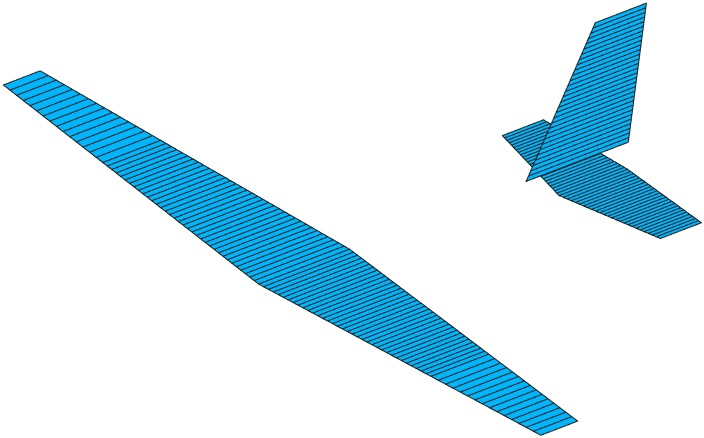
\includegraphics[width=0.7\textwidth]{Images-3-ProjetoDetalhado/vlm_paineis.jpeg} 
    \caption{Divisão dos painéis ao longo da envergadura no CEA-VLM.}
    \label{fig:vlm_paineis}
\end{figure}

Diferentemente de uma análise puramente potencial, que forneceria apenas a inclinação da curva de sustentação e o arrasto induzido linear, o CEA-VLM opera acoplando a solução 3D aos dados viscosos bidimensionais dos perfis aerodinâmicos. O algoritmo interpola as polares 2D dos perfis (coeficientes $C_L$, $C_D$ e $C_m$ em função de $\alpha$ e do número de Reynolds) para cada seção da asa e das empenagens. Este procedimento permite calcular os coeficientes globais tridimensionais de forma não linear, capturando efeitos viscosos como a perda de sustentação (estol) e o aumento do arrasto de perfil.

A geometria foi modelada reproduzindo as características descritas no Capítulo 4, utilizando os perfis NACA 43016 (raiz) e NACA 43009 (ponta) para a asa, e NACA 0012 para as empenagens.

Foram simuladas três condições operacionais distintas, considerando as deflexões de flap pertinentes a cada fase de voo.

O cálculo considerou a geometria completa da aeronave, variando-se o ângulo de ataque global ($\alpha$), mas mantendo a deflexão das superfícies de controle (profundor) nula em todos os pontos. Portanto, os valores representam a capacidade de geração de sustentação e o arrasto associado para a atitude da aeronave, sem o equilíbrio de momentos longitudinais.

O arrasto total apresentado nos gráficos é a soma do arrasto aerodinâmico calculado pelo CEA-VLM (induzido + viscoso da asa/empenagem) com o coeficiente de arrasto parasita da fuselagem e demais componentes ($C_{D_0}$) calculado analiticamente nas Seções 7.2 a 7.4.

As Figuras a seguir apresentam as polares obtidas para as três condições analisadas.

\begin{figure}[H]
    \centering
    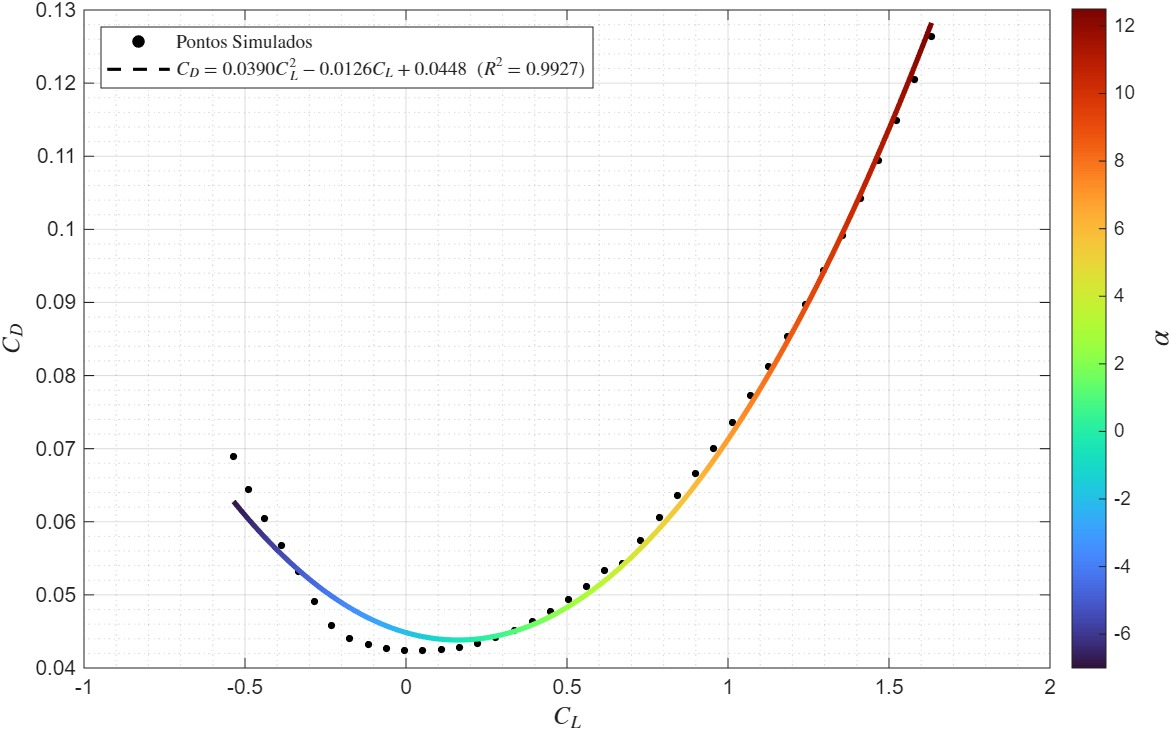
\includegraphics[width=0.7\textwidth]{Images-3-ProjetoDetalhado/polar_cruzeiro.jpeg} 
    \caption{Polar de Arrasto ($C_L \times C_D$) - Condição de Cruzeiro.}
    \label{fig:polar_cruzeiro}
\end{figure}

\begin{figure}[H]
    \centering
    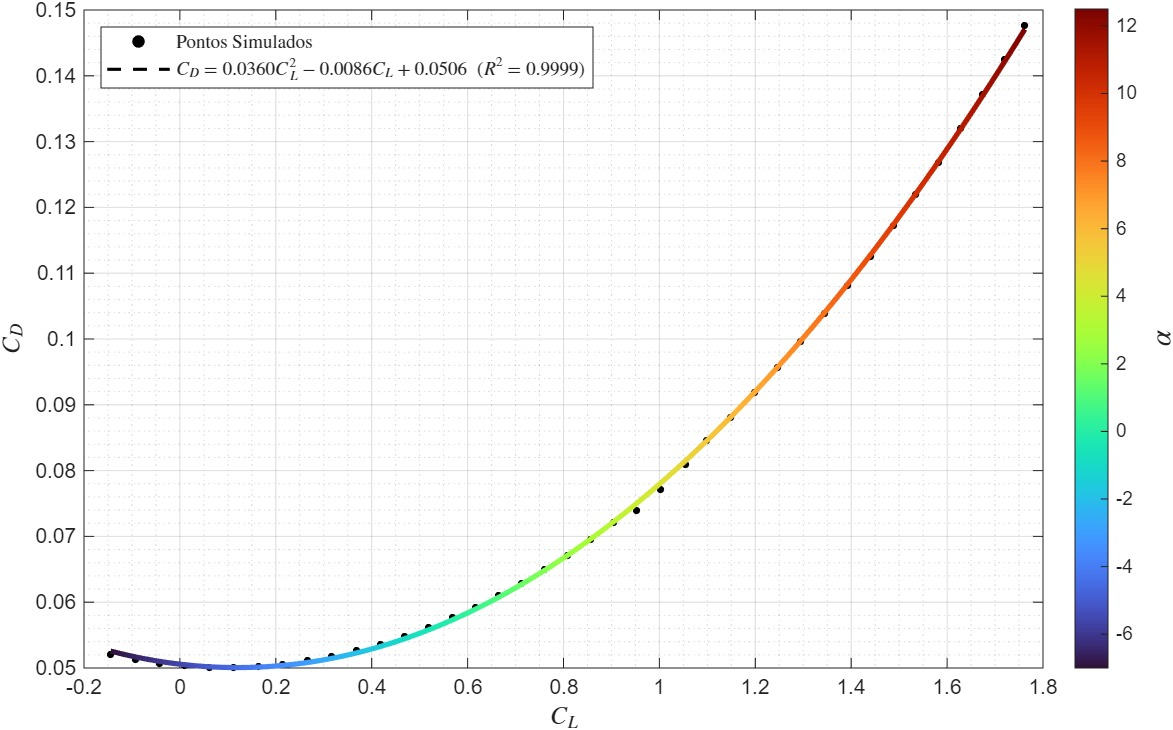
\includegraphics[width=0.7\textwidth]{Images-3-ProjetoDetalhado/polar_decolagem.jpeg}
    \caption{Polar de Arrasto ($C_L \times C_D$) - Condição de Decolagem.}
    \label{fig:polar_decolagem}
\end{figure}

\begin{figure}[H]
    \centering
    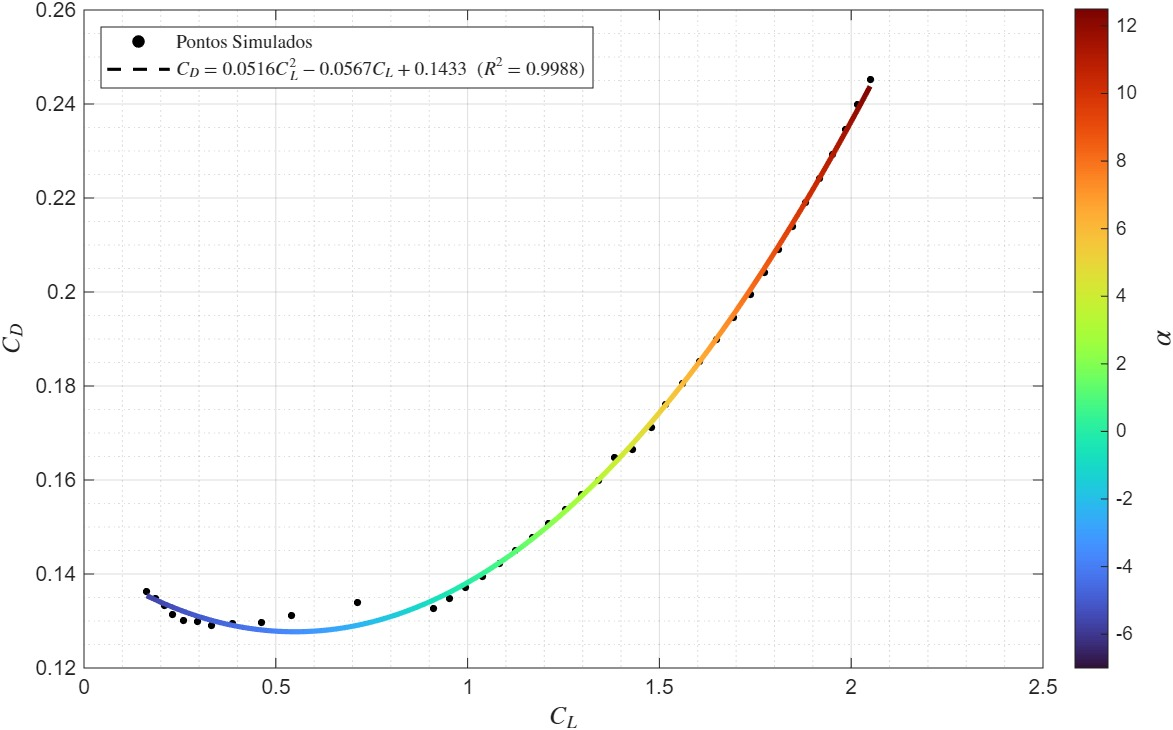
\includegraphics[width=0.7\textwidth]{Images-3-ProjetoDetalhado/polar_pouso.jpeg} 
    \caption{Polar de Arrasto ($C_L \times C_D$) - Condição de Pouso.}
    \label{fig:polar_pouso}
\end{figure}




\section{Cálculo das Potências}

\subsection{Curvas das Potências}

Para realizar os cálculos necessários para obter as curvas de potência \cite{medeiros2017}, foi preciso estimar os valores para 3 condições de voo diferentes, essas são: 

\begin{itemize}
    \item{Decolagem}
    \item{Cruzeiro}
    \item{Pouso}
\end{itemize}

Para traçar cada uma dessas curvas, é preciso obter os valores de potência requerida $P_{req}$ e de potência disponível $P_{disp}$, em relação à variação da velocidade da aeronave em uma determinada altura.

Para as condições de decolagem e cruzeiro, utiliza-se a potência requerida para voo sustentado. No pouso, entretanto, a aeronave encontra-se em trajetória descendente. Assim, a curva correspondente é interpretada como uma condição de planeio, na qual a perda de energia potencial gravitacional contribui para vencer o arrasto.

\subsubsection{Potência requerida:}

Primeiramente, para calcular a potência requerida, pode-se utilizar a seguinte equação que define ela.

\begin{equation}
P_{req} = D.V
\label{eq:preq}
\end{equation}

Na qual, D é a força de arrasto e V é a velocidade de interesse. Portanto, é necessário obter o arrasto e estimar uma velocidade para que o cálculo seja realizado. No entanto, D varia com a velocidade, ou seja, para cada um dos valores de velocidade, D irá variar.

Além disso, considerando que a aeronave estará em voo reto nivelado não acelerado, é possível demonstrar que:

\begin{equation}
C_L = \frac{L}{0.5 \cdot \rho \cdot V^2 \cdot S} = \frac{W}{0.5 \cdot \rho \cdot V^2 \cdot S}
\label{eq:cl}
\end{equation}

Ademais, o arrasto também pode ser definido pela equação utilizando o seu coeficiente:

\begin{equation}
C_D = \frac{D}{0.5 \cdot \rho \cdot V^2 \cdot S}
\label{eq:cd}
\end{equation}

Logo, ao substituir as equações \ref{eq:cl} e \ref{eq:cd} na equação \ref{eq:preq}, é possível chegar na seguinte relação que foi utilizada para traçar a curva de potência requerida pela velocidade:

\begin{equation}
P_{req} = \frac{W.V}{C_L/C_D}
\label{eq:preq2}
\end{equation}

Agora, para o procedimento de cálculo, é necessário que sejam calculados valores de $C_L$ para as diferentes velocidades, por meio da equação \ref{eq:cl}. Ao obter esses valores, pode-se utilizar os dados do gráfico da polar de arrasto para obter os valores de $C_D$ em relação à velocidade. Finalmente, com os valores obtidos, basta variar a V, para se obter o gráfico de interesse. Esse procedimento foi realizado para as 3 condições de voo e os seus cálculos são encontrados abaixo.

É importante notar que a densidade do ar ($\rho$) irá variar conforme a altitude considerada, mas obtendo-se ela os cálculos podem ser realizados.

\begin{itemize}
    \item{Decolagem:}
\end{itemize}

A altitude considerada para os cálculos foi ao nível do mar, ou seja, de acordo com a atmosfera ISA, $\rho = 1,225 \space kg/m^3$. Abaixo encontra-se a tabela com os valores obtidos.


\begin{table}[H]
\centering
\caption{Valores obtidos por meio dos cálculos - Decolagem.}
\begin{tabular}{c c c c}
\hline
Velocidade [m/s] & $C_L$ & $C_D$ & Potência Requerida [kW] \\
\hline
20 & 12{,}2560 & 5{,}3524 & 1943{,}4 \\
30 & 5{,}4469 & 1{,}0718 & 1313{,}4 \\
40 & 3{,}0639 & 0{,}3622 & 1052{,}1 \\
50 & 1{,}9609 & 0{,}1722 & 976{,}7 \\
60 & 1{,}3617 & 0{,}1056 & 1035{,}7 \\
70 & 1{,}0005 & 0{,}0780 & 1214{,}7 \\
80 & 0{,}7660 & 0{,}0651 & 1513{,}6 \\
90 & 0{,}6052 & 0{,}0586 & 1938{,}2 \\
100 & 0{,}4902 & 0{,}0550 & 2497{,}8 \\
110 & 0{,}4051 & 0{,}0530 & 3203{,}1 \\
\hline
\end{tabular}
\end{table}


\begin{itemize}
    \item{Cruzeiro:}
\end{itemize}

A altitude considerada para os cálculos foi à \text{20.000} pés, ou seja, de acordo com a atmosfera ISA, $\rho = \text{0,653} \space kg/m^3$. Abaixo encontra-se a tabela com os valores obtidos.

\begin{table}[H]
\centering
\caption{Valores obtidos por meio dos cálculos - Cruzeiro.}
\begin{tabular}{c c c c}
\hline
Velocidade [m/s] & $C_L$ & $C_D$ & Potência Requerida [kW] \\
\hline
50 & 3{,}6785 & 0{,}5262 & 1591{,}3 \\
60 & 2{,}5545 & 0{,}2671 & 1395{,}9 \\
70 & 1{,}8768 & 0{,}1585 & 1315{,}5 \\
80 & 1{,}4369 & 0{,}1072 & 1328{,}1 \\
90 & 1{,}1354 & 0{,}0808 & 1424{,}5 \\
100 & 0{,}9196 & 0{,}0662 & 1601{,}5 \\
110 & 0{,}7600 & 0{,}0578 & 1859{,}7 \\
120 & 0{,}6386 & 0{,}0527 & 2201{,}5 \\
130 & 0{,}5442 & 0{,}0495 & 2630{,}6 \\
140 & 0{,}4692 & 0{,}0475 & 3151{,}6 \\
150 & 0{,}4087 & 0{,}0462 & 3769{,}5 \\
160 & 0{,}3592 & 0{,}0453 & 4489{,}7 \\
\hline
\end{tabular}
\end{table}


\begin{itemize}
    \item{Pouso:}
\end{itemize}

Os cálculos foram realizados ao nível do mar em atmosfera padrão ($\rho = 1{,}225~\text{kg/m}^3$, ISA), considerando a aeronave no peso máximo de pouso ($\text{MLW} = 22\,350~\text{kgf}$). A Tabela~\ref{tab:pouso_p_req} reúne os resultados obtidos.

\begin{table}[H]
    \centering
    \caption{Valores obtidos por meio dos cálculos - Pouso (MLW).}
    \label{tab:pouso_p_req}
    \begin{tabular}{c c c c}
    \hline
        Velocidade [m/s] & $C_L$ & $C_D$ & Potência dissipada no planeio [kW] \\
    \hline
        20 & 12{,}0771 & 6{,}9769 & 2533{,}2 \\
        30 & 5{,}3676 & 1{,}3264 & 1625{,}4 \\
        40 & 3{,}0193 & 0{,}4429 & 1286{,}5 \\
        50 & 1{,}9323 & 0{,}2266 & 1285{,}4 \\
        60 & 1{,}3419 & 0{,}1602 & 1571{,}0 \\
        70 & 0{,}9859 & 0{,}1376 & 2141{,}7 \\
        80 & 0{,}7548 & 0{,}1299 & 3018{,}4 \\
        90 & 0{,}5964 & 0{,}1279 & 4232{,}2 \\
    \hline
    \end{tabular}
\end{table}

\subsubsection{Potência disponível:}

Primeiramente, é necessário determinar a potência de eixo (SHP) do motor para as três condições de voo analisadas. As potências foram estimadas com base na documentação técnica do motor PW120, pertencente à mesma família do PW127M, conforme a referência \cite{manual_pw120}. Para a decolagem, considerou-se a potência máxima de eixo disponível. Para o cruzeiro, adotou-se 79\% dessa potência e, para o pouso, 40\%, como hipóteses de operação utilizadas na análise de desempenho.


Portanto, os valores de potência no eixo foram estimados para cada condição de voo:

\begin{itemize}
    \item Decolagem:
    \[
        P_{\mathrm{SHP}} = 1{,}00\,P_{\max} = 4950~\mathrm{shp}
    \]

    \item Cruzeiro:
    \[
        P_{\mathrm{SHP}} = 0{,}79\,P_{\max} = 3910{,}5~\mathrm{shp}
    \]

    \item Pouso:
    \[
        P_{\mathrm{SHP}} = 0{,}40\,P_{\max} = 1980~\mathrm{shp}
    \]
\end{itemize}


Após obter o valor de SHP, é necessário considerar a eficiência da hélice para realizar o cálculo da $P_{disp}$, utilizando-se da seguinte relação:

\begin{equation}
    P_{\mathrm{disp}} = \eta_{\mathrm{prop}}\,P_{\mathrm{SHP}}
    \label{eq:pdisp}
\end{equation}

Para isso é necessário utilizar o gráfico da eficiência da hélice em função da razão de avanço da mesma ($J$). Entretanto as curvas de eficiência para a hélice \textit{Hamilton Standard 568F} estão sob sigilo empresarial. Dessa forma, adotaram-se as curvas de eficiência da hélice \textit{Clark Y}. Nesse sentido, a equação da razão de avanço é apresentada a seguir:



\begin{equation}
J = \frac{V}{n \cdot D}
\label{eq:avanco}
\end{equation}


Foi considerado o valor de 1200 rotações por minuto para as três condições de voo, adotando-se um ângulo de pá de 15° para decolagem e pouso e de 30° para cruzeiro. Como a aeronave possui hélices de passo variável, para razões de avanço que ultrapassam os limites das curvas correspondentes aos ângulos de pá definidos, adota-se a maior eficiência disponível. A seguir, apresentam-se as tabelas com os valores da razão de avanço em função da velocidade para cada condição de voo.

\begin{itemize}
    \item{Decolagem:}
\end{itemize}


\begin{table}[H]
\centering
\caption{Razão de avanço $J$ e eficiência $\eta_{\mathrm{prop}}$ em função da velocidade de voo - Decolagem.}
\begin{tabular}{ccc}
\hline
Velocidade [m/s] & $J$ & $\eta_{\mathrm{prop}}$ \\
\hline
20 & 0{,}2545 & 0{,}50 \\
30 & 0{,}3817 & 0{,}65 \\
40 & 0{,}5089 & 0{,}78 \\
50 & 0{,}6361 & 0{,}82 \\
60 & 0{,}7634 & 0{,}84 \\
70 & 0{,}8906 & 0{,}82 \\
80 & 1{,}0178 & 0{,}78 \\
90 & 1{,}1450 & 0{,}73 \\
100 & 1{,}2723 & 0{,}67 \\
110 & 1{,}3995 & 0{,}64 \\
\hline
\end{tabular}
\end{table}


\begin{itemize}
    \item{Cruzeiro:}
\end{itemize}

\begin{table}[H]
\centering
\caption{Razão de avanço $J$ e eficiência $\eta_{\mathrm{prop}}$ em função da velocidade de voo - Cruzeiro.}
\begin{tabular}{ccc}
\hline
Velocidade [m/s] & $J$ & $\eta_{\mathrm{prop}}$ \\
\hline
50 & 0{,}6361 & 0{,}50 \\
60 & 0{,}7634 & 0{,}70 \\
70 & 0{,}8906 & 0{,}78 \\
80 & 1{,}0178 & 0{,}82 \\
90 & 1{,}1450 & 0{,}84 \\
100 & 1{,}2723 & 0{,}85 \\
110 & 1{,}3995 & 0{,}84 \\
120 & 1{,}5267 & 0{,}82 \\
130 & 1{,}6539 & 0{,}81 \\
140 & 1{,}7812 & 0{,}79 \\
150 & 1{,}9084 & 0{,}77 \\
160 & 2{,}0356 & 0{,}75 \\
\hline
\end{tabular}
\end{table}

\clearpage
\begin{itemize}
    \item{Pouso:}
\end{itemize}

\begin{table}[H]
\centering
\caption{Razão de avanço $J$ e eficiência $\eta_{\mathrm{prop}}$ em função da velocidade de voo - Pouso.}
\begin{tabular}{ccc}
\hline
Velocidade [m/s] & $J$ & $\eta_{\mathrm{prop}}$ \\
\hline
20 & 0{,}2545 & 0{,}50 \\
30 & 0{,}3817 & 0{,}65 \\
40 & 0{,}5089 & 0{,}78 \\
50 & 0{,}6361 & 0{,}82 \\
60 & 0{,}7634 & 0{,}84 \\
70 & 0{,}8906 & 0{,}82 \\
80 & 1{,}0178 & 0{,}81 \\
90 & 1{,}1450 & 0{,}80 \\
\hline
\end{tabular}
\end{table}


Com os valores da eficiência e do \textit{Shaft Horsepower}, é possível estimar a potência disponível em função da velocidade para cada uma das condições.

\begin{itemize}
    \item{Decolagem:}
\end{itemize}

\begin{table}[H]
\centering
\caption{Velocidade e potência disponível - Decolagem.}
\begin{tabular}{cc}
\hline
Velocidade [m/s] & Potência disponível [kW] \\
\hline
20 & 1845{,}6 \\
30 & 2399{,}3 \\
40 & 2879{,}2 \\
50 & 3026{,}8 \\
60 & 3100{,}6 \\
70 & 3026{,}8 \\
80 & 2879{,}2 \\
90 & 2694{,}6 \\
100 & 2473{,}1 \\
110 & 2362{,}4 \\
\hline
\end{tabular}
\end{table}

\clearpage

\begin{itemize}
    \item{Cruzeiro:}
\end{itemize}

\begin{table}[H]
\centering
\caption{Velocidade e potência disponível - Cruzeiro.}
\begin{tabular}{cc}
\hline
Velocidade [m/s] & Potência disponível [kW] \\
\hline
50 & 1458{,}0 \\
60 & 2041{,}2 \\
70 & 2274{,}5 \\
80 & 2391{,}2 \\
90 & 2449{,}5 \\
100 & 2478{,}7 \\
110 & 2449{,}5 \\
120 & 2391{,}2 \\
130 & 2362{,}0 \\
140 & 2303{,}7 \\
150 & 2245{,}4 \\
160 & 2187{,}0 \\
\hline
\end{tabular}
\end{table}

\begin{itemize}
    \item{Pouso:}
\end{itemize}

\begin{table}[H]
\centering
\caption{Velocidade e potência disponível - Pouso.}
\begin{tabular}{cc}
\hline
Velocidade [m/s] & Potência disponível [kW] \\
\hline
20 & 738{,}24 \\
30 & 959{,}72 \\
40 & 1151{,}7 \\
50 & 1210{,}7 \\
60 & 1240{,}2 \\
70 & 1210{,}7 \\
80 & 1196{,}0 \\
90 & 1181{,}2 \\
\hline
\end{tabular}
\end{table}

\subsubsection{Gráficos obtidos}

Finalmente, com todos os valores obtidos pelos cálculos, foi possível traçar os gráficos necessários. Todos os 3 podem ser encontrados abaixo.

\clearpage

\begin{itemize}
    \item{Decolagem:}
\end{itemize}

\begin{figure}[H]
    \centering
    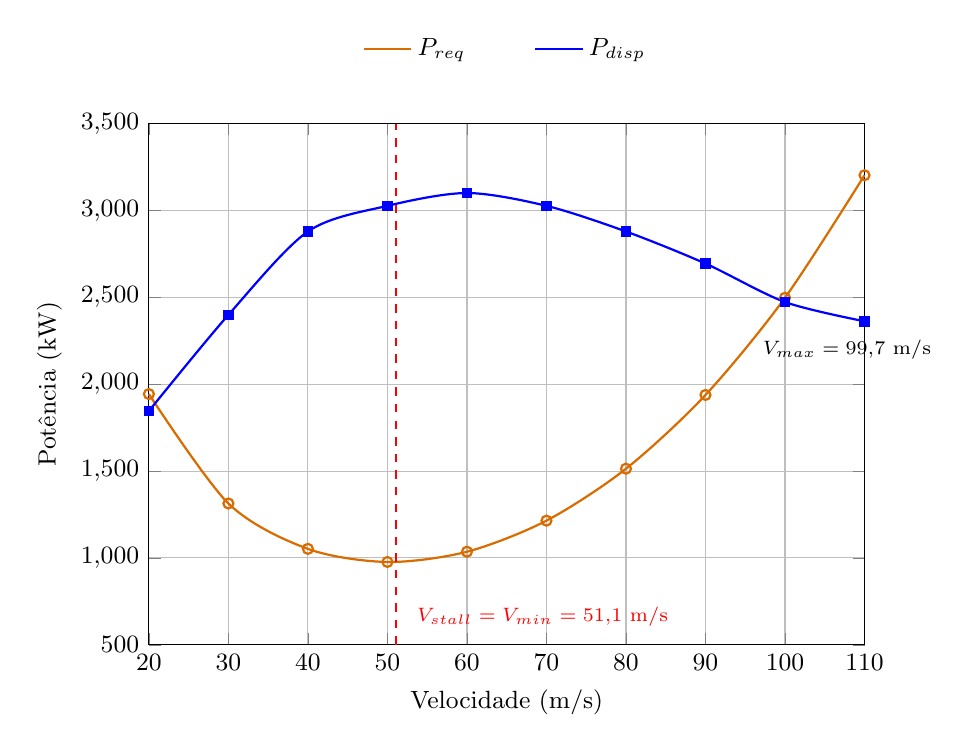
\begin{tikzpicture}
    \begin{axis}[
        width=0.88\textwidth,
        height=8.2cm,
        xlabel={Velocidade (m/s)},
        ylabel={Potência (kW)},
        xmin=20, xmax=110,
        ymin=500, ymax=3500,
        grid=major,
        tick label style={font=\small},
        label style={font=\small},
        legend columns=2,
        legend style={
            at={(0.5,1.10)},
            anchor=south,
            font=\small,
            draw=none,
            fill=none,
            /tikz/every even column/.append style={column sep=0.8cm}
        },
        clip=false,
        every axis plot/.append style={thick}
    ]

    % Potência requerida (Tabela 7.10, MTOW)
    \addplot[color=orange!85!black, smooth, mark=none] coordinates {
        (20,1943.4) (30,1313.4) (40,1052.1) (50,976.7) (60,1035.7)
        (70,1214.7) (80,1513.6) (90,1938.2) (100,2497.8) (110,3203.1)
    };
    \addlegendentry{$P_{req}$}
    \addplot[only marks, color=orange!85!black, mark=o, mark options={scale=0.9}, forget plot] coordinates {
        (20,1943.4) (30,1313.4) (40,1052.1) (50,976.7) (60,1035.7)
        (70,1214.7) (80,1513.6) (90,1938.2) (100,2497.8) (110,3203.1)
    };

    % Potência disponível (Tabela 7.16)
    \addplot[color=blue, smooth, mark=none] coordinates {
        (20,1845.6) (30,2399.3) (40,2879.2) (50,3026.8) (60,3100.6)
        (70,3026.8) (80,2879.2) (90,2694.6) (100,2473.1) (110,2362.4)
    };
    \addlegendentry{$P_{disp}$}
    \addplot[only marks, color=blue, mark=square*, mark options={scale=0.75}, forget plot] coordinates {
        (20,1845.6) (30,2399.3) (40,2879.2) (50,3026.8) (60,3100.6)
        (70,3026.8) (80,2879.2) (90,2694.6) (100,2473.1) (110,2362.4)
    };

    % Velocidade de estol com flap 10° (Seção 7.6)
    \addplot[red, dashed, thick] coordinates {(51.1,500) (51.1,3500)};

    % Anotações
    \node[red, anchor=west, font=\scriptsize] at (axis cs:52.5,660)
        {$V_{stall}=V_{min}=51{,}1\ \mathrm{m/s}$};
    \node[anchor=west, font=\scriptsize] at (axis cs:96,2200)
        {$V_{max}=99{,}7\ \mathrm{m/s}$};

    \end{axis}
    \end{tikzpicture}
    \caption{Curvas de potência na decolagem com $10^\circ$ de flap (nível do mar, 100\% SHP, MTOW).}
    \label{fig:potencia_decolagem_suave}
\end{figure}

Para uma análise com mais detalhes, sugere-se também a análise das curvas sem deflexão dos flaps, haja vista que para velocidades altas algumas aeronaves podem não acionar os flaps na decolagem.


\clearpage


\begin{itemize}
    \item{Cruzeiro:}
\end{itemize}

\begin{figure}[H]
    \centering
    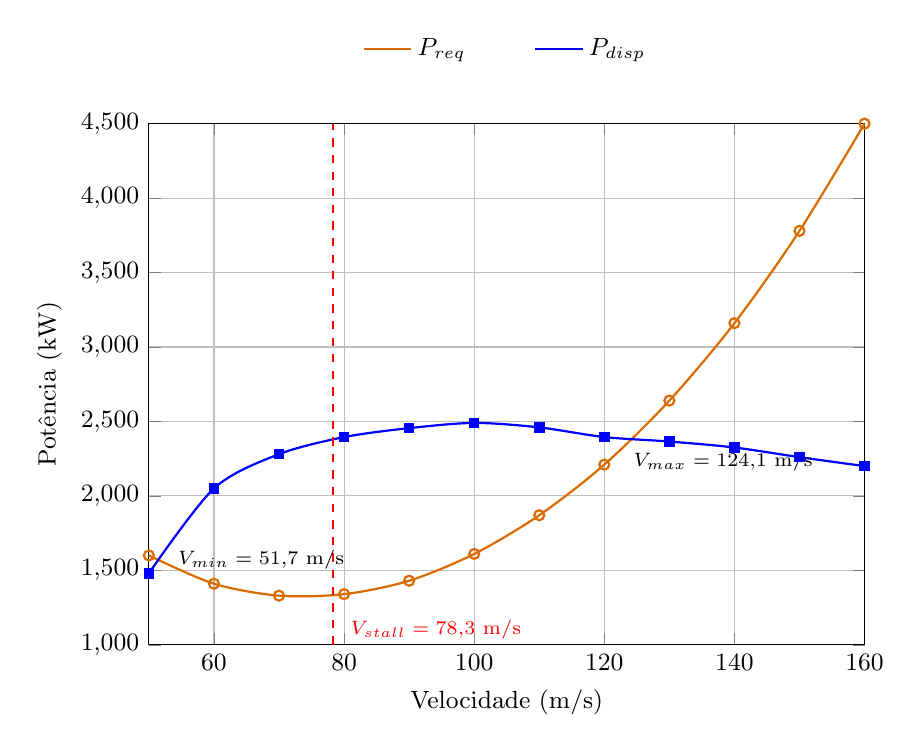
\begin{tikzpicture}
    \begin{axis}[
        width=0.88\textwidth,
        height=8.2cm,
        xlabel={Velocidade (m/s)},
        ylabel={Potência (kW)},
        xmin=50, xmax=160,
        ymin=1000, ymax=4500,
        grid=major,
        tick label style={font=\small},
        label style={font=\small},
        legend columns=2,
        legend style={
            at={(0.5,1.10)},
            anchor=south,
            font=\small,
            draw=none,
            fill=none,
            /tikz/every even column/.append style={column sep=0.8cm}
        },
        clip=false,
        every axis plot/.append style={thick}
    ]

    % -------------------------
    % Potência requerida
    % -------------------------
    \addplot[
        color=orange!85!black,
        smooth,
        mark=none
    ] coordinates {
        (50,1600)
        (60,1410)
        (70,1330)
        (80,1340)
        (90,1430)
        (100,1610)
        (110,1870)
        (120,2210)
        (130,2640)
        (140,3160)
        (150,3780)
        (160,4500)
    };
    \addlegendentry{$P_{req}$}

    \addplot[
        only marks,
        color=orange!85!black,
        mark=o,
        mark options={scale=0.9},
        forget plot
    ] coordinates {
        (50,1600)
        (60,1410)
        (70,1330)
        (80,1340)
        (90,1430)
        (100,1610)
        (110,1870)
        (120,2210)
        (130,2640)
        (140,3160)
        (150,3780)
        (160,4500)
    };

    % -------------------------
    % Potência disponível
    % -------------------------
    \addplot[
        color=blue,
        smooth,
        mark=none
    ] coordinates {
        (50,1480)
        (60,2050)
        (70,2280)
        (80,2395)
        (90,2455)
        (100,2490)
        (110,2460)
        (120,2395)
        (130,2365)
        (140,2325)
        (150,2260)
        (160,2200)
    };
    \addlegendentry{$P_{disp}$}

    \addplot[
        only marks,
        color=blue,
        mark=square*,
        mark options={scale=0.75},
        forget plot
    ] coordinates {
        (50,1480)
        (60,2050)
        (70,2280)
        (80,2395)
        (90,2455)
        (100,2490)
        (110,2460)
        (120,2395)
        (130,2365)
        (140,2325)
        (150,2260)
        (160,2200)
    };

    % -------------------------
    % Linha da velocidade de estol
    % -------------------------
    \addplot[
        red,
        dashed,
        thick
    ] coordinates {(78.3,1000) (78.3,4500)};

    % -------------------------
    % Anotações
    % -------------------------
    \node[anchor=west, font=\scriptsize] at (axis cs:53,1570)
        {$V_{min}=51{,}7\ \mathrm{m/s}$};

    \node[red, anchor=west, font=\scriptsize] at (axis cs:79.5,1100)
        {$V_{stall}=78{,}3\ \mathrm{m/s}$};

    \node[anchor=west, font=\scriptsize] at (axis cs:123,2230)
        {$V_{max}=124{,}1\ \mathrm{m/s}$};

    \end{axis}
    \end{tikzpicture}
    \caption{Curvas de potência no cruzeiro (20.000 ft, 79\% SHP).}
    \label{fig:potencia_cruzeiro_suave}
\end{figure}


\begin{itemize}
    \item{Pouso:}
\end{itemize}

\begin{figure}[H]
    \centering
    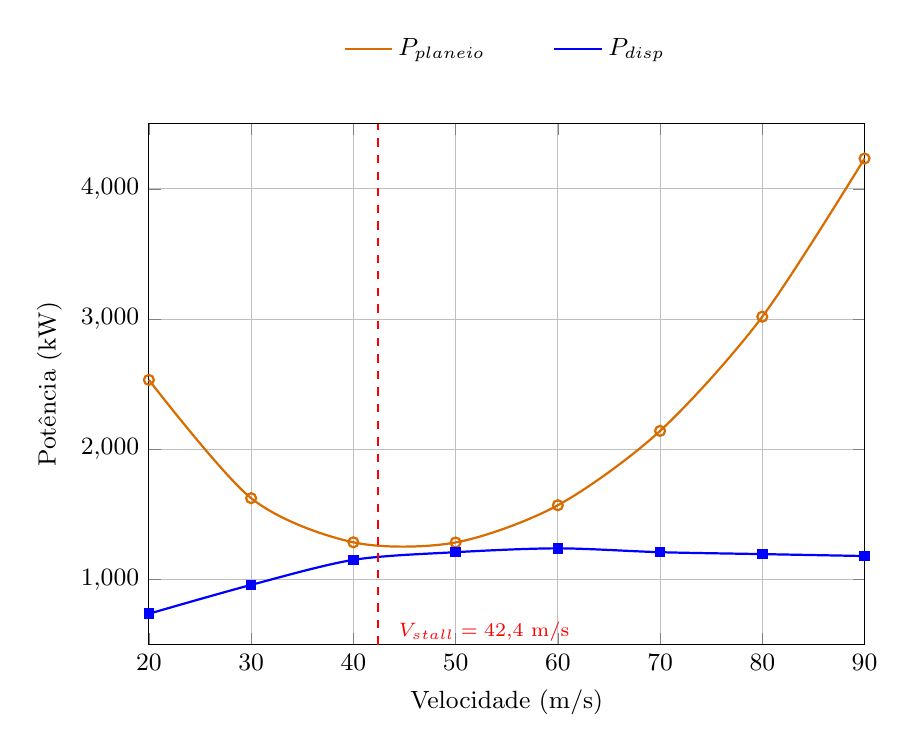
\begin{tikzpicture}
    \begin{axis}[
        width=0.88\textwidth,
        height=8.2cm,
        xlabel={Velocidade (m/s)},
        ylabel={Potência (kW)},
        xmin=20, xmax=90,
        ymin=500, ymax=4500,
        grid=major,
        tick label style={font=\small},
        label style={font=\small},
        legend columns=2,
        legend style={
            at={(0.5,1.10)},
            anchor=south,
            font=\small,
            draw=none,
            fill=none,
            /tikz/every even column/.append style={column sep=0.8cm}
        },
        clip=false,
        every axis plot/.append style={thick}
    ]

    % Condição de planeio (Tabela 7.12, MLW)
    \addplot[color=orange!85!black, smooth, mark=none] coordinates {
        (20,2533.2) (30,1625.4) (40,1286.5) (50,1285.4)
        (60,1571.0) (70,2141.7) (80,3018.4) (90,4232.2)
    };
    \addlegendentry{$P_{planeio}$}
    \addplot[only marks, color=orange!85!black, mark=o, mark options={scale=0.9}, forget plot] coordinates {
        (20,2533.2) (30,1625.4) (40,1286.5) (50,1285.4)
        (60,1571.0) (70,2141.7) (80,3018.4) (90,4232.2)
    };

    % Potência disponível (Tabela 7.18)
    \addplot[color=blue, smooth, mark=none] coordinates {
        (20,738.2) (30,959.7) (40,1151.7) (50,1210.7)
        (60,1240.2) (70,1210.7) (80,1196.0) (90,1181.2)
    };
    \addlegendentry{$P_{disp}$}
    \addplot[only marks, color=blue, mark=square*, mark options={scale=0.75}, forget plot] coordinates {
        (20,738.2) (30,959.7) (40,1151.7) (50,1210.7)
        (60,1240.2) (70,1210.7) (80,1196.0) (90,1181.2)
    };

    % Velocidade de estol com flap 40°, MLW (Seção 7.6)
    \addplot[red, dashed, thick] coordinates {(42.4,500) (42.4,4500)};

    % Anotações
    \node[red, anchor=west, font=\scriptsize] at (axis cs:43.5,600)
        {$V_{stall}=42{,}4\ \mathrm{m/s}$};

    \end{axis}
    \end{tikzpicture}
    \caption{Condição de planeio e potência disponível no pouso com $40^\circ$ de flap (nível do mar, 40\% SHP, MLW).}
    \label{fig:potencia_pouso_suave}
\end{figure}

Assim como comentado nas curvas de potência para decolagem, no pouso sugere-se, em análises posteriores, a verificação de pouso sem deflexão dps flaps e/ou com angulações menores.

\section{Velocidades Máximas, Mínimas e Estol}

A velocidade máxima e mínima de voo em cada condição podem ser determinadas por meio dos gráficos de velocidade x potência. Quando a curva de potência requerida cruza a curva de potência disponível, sabe-se que são nesses pontos que se encontram as velocidades mínimas e máximas de operação, entretanto quando a velocidade mínima através da interseção das curvas é inferior a de estol, a velocidade de estol é a mínima de voo, abaixo encontram-se os valores obtidos para as 3 condições.

\begin{itemize}
    \item{Decolagem:}
\end{itemize}

\begin{equation}
    V_{min,decolagem} = 51{,}1 \text{ m/s} = 99{,}3 \text{ kt}
\end{equation}

\begin{equation}
    V_{max,decolagem} = 99{,}7 \text{ m/s} = 193{,}8 \text{ kt}
\end{equation}


\begin{itemize}
    \item{Cruzeiro:}
\end{itemize}


\begin{equation}
    V_{min,cruzeiro} = 78{,}3 \text{ m/s} = 152{,}2 \text{ kt}
\end{equation}

\begin{equation}
    V_{max,cruzeiro} = 124{,}1 \text{ m/s} = 241{,}3 \text{ kt}
\end{equation}

\begin{itemize}
    \item Pouso:
\end{itemize}

Na condição de pouso, não se utiliza a interseção entre potência requerida e potência disponível para determinar os limites de velocidade, pois a aeronave encontra-se em trajetória descendente. A aproximação é tratada como uma condição de planeio, na qual a perda de energia potencial contribui para vencer o arrasto. Dessa forma, a velocidade de aproximação é definida a partir da velocidade de estol e dos fatores de segurança adotados para o pouso.

\begin{itemize}
    \item \textbf{Velocidade de Estol:}
\end{itemize}

As velocidades de estol para cada condição operacional são determinadas pela Equação~5.10, empregando o peso correspondente à fase de voo (Tabela~\ref{tab:cg_entradas}) e os coeficientes de sustentação máximos de cada configuração aerodinâmica ($C_{L\max} = 1{,}50$ em configuração limpa, $1{,}88$ com flap a $10^\circ$ e $2{,}69$ com flap a $40^\circ$, valores consistentes com o diagrama $V\text{--}n$ da Seção~9.2). Cabe ressaltar que os coeficientes de $1{,}17$ e $1{,}59$ reportados na Tabela~5.2 correspondem às condições operacionais de decolagem ($1{,}13\,V_S$) e pouso ($1{,}30\,V_S$), e não aos limites de estol.

\begin{itemize}
    \item \textbf{Pouso (nível do mar, flap $40^\circ$, MLW):}
    \begin{equation}
        V_{S,L} = \sqrt{\frac{2 \cdot 22\,350 \cdot 9{,}81}{1{,}225 \cdot 74{,}1 \cdot 2{,}69}} = 42{,}4~\text{m/s} \approx 82{,}4~\text{kt}
    \end{equation}

    \item \textbf{Decolagem (nível do mar, flap $10^\circ$, MTOW):}
    \begin{equation}
        V_{S,TO} = \sqrt{\frac{2 \cdot 22\,680 \cdot 9{,}81}{1{,}225 \cdot 74{,}1 \cdot 1{,}88}} = 51{,}1~\text{m/s} \approx 99{,}3~\text{kt}
    \end{equation}

    \item \textbf{Configuração limpa (MTOW):} $V_S = 57{,}2~\text{m/s}$ ($111~\text{kt}$) ao nível do mar, conforme a Tabela~5.2, atingindo $V_S = 78{,}3~\text{m/s}$ ($152{,}2~\text{kt}$ TAS) a $20\,000~\text{ft}$ ($\rho = 0{,}653~\text{kg/m}^3$).
\end{itemize}

A partir desses limites, obtêm-se a velocidade operacional de aproximação ($1{,}30\,V_{S,L} = 55{,}1~\text{m/s}$ ou $107{,}1~\text{kt}$) e a velocidade de decolagem de $125~\text{kt}$ apresentada na Tabela~5.2.


\section{Distância de Decolagem}

A avaliação do desempenho de decolagem do turboélice regional fundamenta-se nos requisitos de certificação da categoria transporte estabelecidos pelo 14 CFR Part~25 e pelo RBAC~25~\cite{far25}. Os cálculos consideram operação ao nível do mar em atmosfera padrão (ISA), com os motores em potência máxima de decolagem, a aeronave em seu peso máximo de decolagem (MTOW) e coeficiente de atrito de rolamento $\mu = 0{,}02$, representativo de pista seca de concreto.

Pelo \S25.113, a distância de decolagem corresponde ao maior valor entre o percurso até $35~\text{ft}$ com falha do motor crítico (OEI) e $115\%$ do percurso até a mesma altura com todos os motores operantes (AEO). Complementarmente, o \S25.109 define a distância de aceleração-parada para o caso de decolagem abortada após a falha. Nas subseções seguintes, determina-se inicialmente o desempenho com todos os motores operando (Seções~7.7.1 a 7.7.3) e, na sequência, analisa-se a condição monomotora por meio do comprimento de pista balanceado (BFL), na Seção~7.7.4.

Os critérios normativos aplicáveis estão esquematizados na Figura~\ref{fig:fases_decolagem}.

\begin{figure}[H]
\centering
\resizebox{\textwidth}{!}{%
\begin{tikzpicture}[x=1cm,y=1cm,font=\small,
  dim/.style={{Latex[length=2mm]}-{Latex[length=2mm]},thin},
  vline/.style={densely dotted,gray}]
  % pista
  \fill[gray!15] (0,-0.12) rectangle (14.6,0);
  \draw[thick] (0,0) -- (14.6,0);
  % altura de 35 ft
  \draw[gray,dashed] (0,1.6) -- (14.6,1.6);
  \node[gray,anchor=west] at (12.25,1.85) {35 ft (10,7 m)};
  % todos os motores operando (AEO)
  \draw[very thick,blue!70!black] (0,0) -- (5.4,0)
     .. controls (6.6,0.05) and (7.4,0.9) .. (8.4,1.6) -- (9.0,2.0);
  % motor crítico inoperante (OEI)
  \draw[very thick,red!75!black,dashed] (3.2,0.03) -- (7.2,0.03)
     .. controls (8.6,0.08) and (9.9,0.95) .. (11.0,1.6) -- (11.8,2.0);
  % aceleração-parada
  \draw[very thick,green!45!black,dash dot] (4.0,-0.35) -- (11.0,-0.35);
  \draw[green!45!black] (4.0,-0.2) -- (4.0,-0.5);
  \fill[green!45!black] (11.0,-0.35) circle (1.8pt);
  \node[green!45!black,anchor=north,font=\footnotesize] at (7.5,-0.38) {Frenagem após $V_1$ (parada)};
  % marcas de velocidade
  \draw[vline] (3.2,0) -- (3.2,2.6) node[above] {$V_{EF}$};
  \draw[vline] (4.0,0) -- (4.0,2.6) node[above] {$V_1$};
  \draw[vline] (5.4,0) -- (5.4,2.6) node[above] {$V_{LOF}$};
  \draw[vline] (11.0,0) -- (11.0,2.6) node[above] {$V_2$};
  \node[blue!70!black,anchor=east] at (7.3,1.2) {AEO};
  \node[red!75!black,anchor=west] at (10.0,0.55) {OEI};
  % cotas
  \draw[dim] (0,-1.1) -- (8.4,-1.1) node[midway,fill=white,inner sep=1pt] {$d_{AEO}$ (até 35 ft)};
  \draw[dim] (0,-1.65) -- (9.66,-1.65) node[midway,fill=white,inner sep=1pt] {$1{,}15\,d_{AEO}$};
  \draw[dim] (0,-2.2) -- (11.0,-2.2) node[midway,fill=white,inner sep=1pt] {$d_{OEI}$: Falha do motor crítico em $V_{EF}$ (§25.113(a)(1))};
  \draw[dim] (0,-2.75) -- (11.0,-2.75) node[midway,fill=white,inner sep=1pt] {Distância de aceleração--parada (§25.109)};
  % linhas de chamada das cotas
  \draw[thin,gray] (0,-0.6)    -- (0,-2.9);
  \draw[thin,gray] (8.4,-0.8)  -- (8.4,-1.2);
  \draw[thin,gray] (9.66,-0.8) -- (9.66,-1.75);
  \draw[thin,gray] (11.0,-0.5) -- (11.0,-2.9);
  % legenda lateral
  \node[anchor=west,align=left,font=\footnotesize] at (11.4,-1.9)
     {Distância de decolagem\\$=\max\{d_{OEI};\,1{,}15\,d_{AEO}\}$\\[2pt]
      BFL: $d_{OEI} = $ Dist. de\\aceleração--parada};
\end{tikzpicture}%
}
\caption{Distâncias de decolagem da categoria transporte (alturas fora de escala). Elaborado pelos autores com base no 14 CFR Part 25, §25.109 e §25.113 \cite{far25}.}
\label{fig:fases_decolagem}
\end{figure}

\subsection{Corrida no Solo}
O deslocamento inicial da aeronave sobre a pista, do repouso até $V_{lof}$ na Figura~\ref{fig:fases_decolagem}, define a corrida de decolagem. A velocidade de decolagem ($V_{lof}$) é estimada pela seguinte proporção empírica em relação ao limite de estol:
\begin{equation}
    V_{lof} = 1,13 \cdot V_{s}
\end{equation}
\begin{equation}
    V_{lof} = 125 \text{ kt}= 64,3 \text{ m/s}
\end{equation}

A modelagem dinâmica dessa fase baseia-se na aplicação da Segunda Lei de Newton, equacionando as forças nos eixos horizontal e vertical durante a aceleração da aeronave:
\begin{equation}
    T - D - \mu(W - L) = \frac{W}{g} \cdot \frac{dV}{dt}
\end{equation}
\begin{equation}
    N = W - L
\end{equation}

Sabendo que a aceleração instantânea pode ser reescrita em função do espaço percorrido:
\begin{equation}
    a = \frac{dV}{dt} = \frac{1}{2}\frac{dV^{2}}{dS}
\end{equation}

Isolando o diferencial de espaço e integrando o movimento do repouso até o \textit{lift-off}, encontra-se a distância total de corrida no solo ($S$), conforme a Equação \ref{eq:dist_corrida}:
\begin{equation}
    S = \int_{0}^{V_{LOF}} \frac{W}{2g(T - D)} dV^{2}
    \label{eq:dist_corrida}
\end{equation}

Implementando um algoritmo de integração numérica iterativa, o espaço de corrida calculado foi de:
\begin{equation}
    S = 907,46 \text{ m}
\end{equation}

\subsection{Subida de Decolagem}
Para estimar as distâncias na subida de decolagem, o cálculo foi dividido em duas etapas. A primeira ($S_{1}$) descreve a trajetória curva de transição, modelada como um arco de círculo. O segmento subsequente ($S_{2}$) retrata o trecho de ascensão em trajetória retilínea até o momento em que o trem de pouso cruza a altura estipulada do obstáculo virtual. A geometria dessa transição está demonstrada na Figura \ref{fig:subida_decolagem}.

\begin{figure}[H]
    \centering
    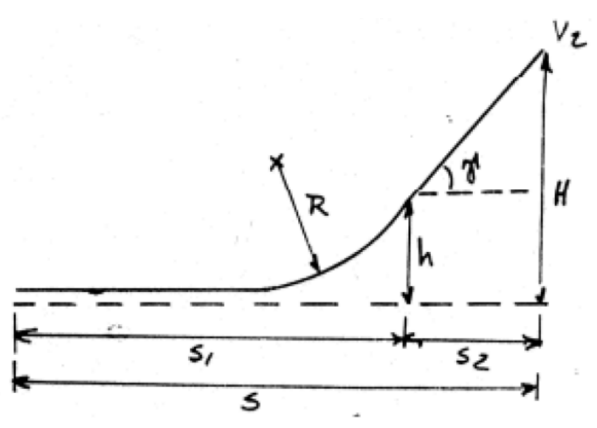
\includegraphics[width=0.6\textwidth]{Images-3-ProjetoDetalhado/subida_decolagem.png} 
    \caption{Subida de decolagem inicial.}
    \label{fig:subida_decolagem}
\end{figure}

Conforme sugerido por Gudmundsson \cite{Gudmundsson}, a velocidade característica ao longo da manobra de arredondamento obedece à relação apresentada na Equação \ref{eq:v_inf}:
\begin{equation}
    V_{\infty} = 1,2 \cdot V_{S}
    \label{eq:v_inf}
\end{equation}
\begin{equation}
    V_{\infty} = 67,1 \text{ m/s}
\end{equation}

O equilíbrio dinâmico radial durante o arco de trajetória é então expresso por:
\begin{equation}
    F_{R} = m \cdot a = m\frac{V_{\infty}^{2}}{R} = L - W \cos \theta
\end{equation}

Como o ângulo da trajetória em relação à horizontal ($\theta$) é pequeno, assume-se que $\cos \theta \approx 1$. Com esta simplificação geométrica, o raio da curva de transição ($R$) é isolado na Equação \ref{eq:raio_subida}:
\begin{equation}
    R = \frac{V_{\infty}^{2}}{g(n - 1)}
    \label{eq:raio_subida}
\end{equation}

Considerando a premissa aerodinâmica de que o $C_{L}$ da manobra atinge cerca de $0,9 \cdot C_{L_{max}}$, considerou-se que o fator de carga para a curva de decolagem é de:
\begin{equation}
    n = \frac{L}{W} = 1,3
\end{equation}

Aplicando este coeficiente na Equação \ref{eq:raio_subida}, obtém-se o raio da trajetória de subida:
\begin{equation}
    R = 1529,9 \text{ m}
\end{equation}

A projeção horizontal da distância percorrida durante esta manobra em arco ($S_{1}$) é obtida geometricamente pela Equação \ref{eq:s1}:
\begin{equation}
    S_{1} = R \cdot \sin \gamma
    \label{eq:s1}
\end{equation}
\begin{equation}
    S_{1} = 122,71 \text{ m}
\end{equation}

Onde $\gamma$ representa o ângulo máximo de subida, estimado pelo balanço de forças longitudinais:
\begin{equation}
    \gamma = \sin^{-1}\left(\frac{T - D}{W}\right) \approx 4,6 ^\circ
\end{equation}

O ganho de altitude correspondente a este segmento ($h$) pode ser aproximado pela correlação geométrica expressa na Equação \ref{eq:altura_transicao}:
\begin{equation}
    h = \frac{S_{1}^{2}}{2 \cdot R}
    \label{eq:altura_transicao}
\end{equation}
\begin{equation}
    h = 4,92 \text{ m}
\end{equation}

Em seguida, o segmento $S_{2}$ é computado admitindo-se uma taxa de subida constante até passar de um obstáculo padrão ($H$) definido pelo 14 CFR Part 25. Fixou-se, então, $H = 35 \text{ ft (10,66 m)}$. O espaço horizontal deste trecho retilíneo torna-se, portanto:
\begin{equation}
    S_{2} = \frac{H - h}{\tan \gamma}
\end{equation}
\begin{equation}
    S_{2} = 71,42 \text{ m}
\end{equation}

\subsection{Distância Total de Decolagem}
Por fim, o comprimento exigido de pista para que a aeronave complete toda a operação de decolagem em segurança é a somatória das etapas elucidadas:
\begin{equation}
    S_{decolagem} = S + S_{1} + S_{2}
\end{equation}
\begin{equation}
    S_{decolagem} = 1101,59\text{ m}
\end{equation}

Esse valor corresponde à decolagem com todos os motores operando. A verificação do requisito de 4 200 ft (1 280 m), no entanto, é feita pela condição monomotora, apresentada na Seção 7.7.4.

\subsection{Comprimento de Pista Balanceado (BFL)}
\label{sec:bfl}
O comprimento de pista balanceado (\emph{Balanced Field Length} -- BFL) corresponde ao comprimento para o qual a interrupção da decolagem e sua continuação após a falha do motor crítico exigem a mesma distância. Sua estimativa foi realizada pelo método semiempírico de Raymer \cite{raymer2018}, considerando atmosfera ISA ao nível do mar, pista seca e horizontal, ausência de vento e peso máximo de decolagem de $22\,680~\mathrm{kgf}$. Foram utilizadas a geometria e as características propulsivas apresentadas anteriormente, adotando-se o valor de $C_{L_{\max,TO}}$ retirado da polar de decolagem.

A velocidade de subida inicial e o coeficiente de sustentação correspondente foram determinados por:
\begin{equation}
    V_2 = 1{,}2
    \sqrt{\frac{2W}{\rho S C_{L_{\max,TO}}}},
    \qquad
    C_{L,\mathrm{sub}} =
    \frac{C_{L_{\max,TO}}}{1{,}2^2}.
\end{equation}

Para a subida monomotor, consideraram-se o trem de pouso recolhido e a hélice do motor inoperante embandeirada. O coeficiente de arrasto foi obtido corrigindo a polar de decolagem:
\begin{equation}
    C_{D,\mathrm{OEI}} =
    C_{D,\mathrm{TO}}(C_{L,\mathrm{sub}})
    - \Delta C_{D,\mathrm{LG}}
    + \Delta C_{D,\text{hélice}}.
\end{equation}

O arrasto e a tração do motor remanescente foram calculados por:
\begin{equation}
    D_{\mathrm{OEI}} =
    \frac{1}{2}\rho V_2^2 S C_{D,\mathrm{OEI}},
    \qquad
    T_{\mathrm{OEI}} =
    \frac{\eta_p P_{\mathrm{eixo},1}}{V_2},
\end{equation}
com a eficiência propulsiva interpolada na velocidade $V_2$. O ângulo de subida resultante é:
\begin{equation}
    \gamma_{\mathrm{OEI}} =
    \arcsin\left(
    \frac{T_{\mathrm{OEI}}-D_{\mathrm{OEI}}}{W}
    \right),
\end{equation}
correspondente a um gradiente de subida estimado de $3{,}29\%$.

A expressão de Raymer, convertida para fornecer a BFL em metros com as demais grandezas no Sistema Internacional, é:
\begin{equation}
    \mathrm{BFL} =
    \frac{0{,}863}{1+2{,}3G}
    \left(
    \frac{W/S}{\rho g C_{L,\mathrm{sub}}}
    + h_{\mathrm{obs}}
    \right)
    \left[
    \frac{1}{T_{\mathrm{av}}/W-U}+2{,}7
    \right]
    + \frac{199{,}64}{\sqrt{\sigma}},
    \label{eq:bfl_raymer}
\end{equation}
em que $\sigma=\rho/\rho_{SL}$, $h_{\mathrm{obs}}=35~\mathrm{ft}=10{,}668~\mathrm{m}$ é a altura de referência e os parâmetros auxiliares são:
\begin{equation}
    G = \gamma_{\mathrm{OEI}}-0{,}024,
    \qquad
    U = 0{,}01C_{L_{\max,TO}}+0{,}02,
\end{equation}
utilizando-se $\gamma_{\mathrm{OEI}}$ em radianos.

A tração média equivalente durante a aceleração foi estimada pela correlação para aeronaves a hélice:
\begin{equation}
    T_{\mathrm{av}} =
    5{,}75P
    \left(
    \frac{\sigma N_e D_p^2}{P}
    \right)^{1/3},
\end{equation}
na qual $P$ é a potência total de eixo em hp, $D_p$ é o diâmetro da hélice em pés e $N_e$ é o número de motores. A tração obtida em lbf foi convertida para newtons antes da aplicação na Equação~\ref{eq:bfl_raymer}.

Os valores intermediários empregados na Equação~\ref{eq:bfl_raymer} estão reunidos na Tabela~\ref{tab:parametros_bfl}.

\begin{table}[H]
    \centering
    \caption{Parâmetros da estimativa do comprimento de pista balanceado (ISA, nível do mar, MTOW).}
    \label{tab:parametros_bfl}
    \begin{tabular}{l c c}
    \toprule
        Grandeza & Símbolo & Valor \\
    \midrule
        Peso de decolagem & $W$ & $22\,680~\text{kgf}$ ($222{,}5~\text{kN}$) \\
        Carga alar & $W/S$ & $3\,003~\text{N/m}^2$ \\
        Coeficiente de sustentação máximo (flap $10^\circ$) & $C_{L\max,TO}$ & $1{,}77$ \\
        Velocidade de segurança de decolagem & $V_2$ & $63{,}1~\text{m/s}$ ($122{,}6~\text{kt}$) \\
        Coeficiente de sustentação na subida & $C_{L,\text{sub}}$ & $1{,}23$ \\
        Gradiente de subida monomotor & $\gamma_{OEI}$ & $3{,}29\%$ \\
        Parâmetros auxiliares & $G\,;\,U$ & $0{,}0089\,;\,0{,}0377$ \\
        Tração média na aceleração & $T_{av}$ & $51{,}5~\text{kN}$ \\
        Razão tração média--peso & $T_{av}/W$ & $0{,}231$ \\
    \midrule
        Comprimento de pista balanceado & BFL & $1\,620~\text{m}$ ($5\,315~\text{ft}$) \\
    \bottomrule
    \end{tabular}
\end{table}

O gradiente monomotor de $3{,}29\%$ atende ao mínimo de $2{,}4\%$ exigido pelo \S25.121(b) para bimotores no segundo segmento \cite{far25}. Quanto ao comprimento de pista, os parágrafos \S25.109 e \S25.113 determinam que a distância de decolagem considere tanto a aceleração-parada quanto o maior valor entre a trajetória monomotora até $35~\mathrm{ft}$ e $115\%$ da distância com todos os motores operantes \cite{far25}. Como o caso normal majorado ($1{,}15 \times 1\,101{,}6 = 1\,267~\mathrm{m}$) permanece abaixo do limite, a restrição decorre da condição monomotora, representada pela BFL:
\begin{equation}
    \mathrm{BFL} \approx 1\,620~\mathrm{m} \;>\; 1\,280~\mathrm{m}~(4\,200~\mathrm{ft})
\end{equation}
valor $26{,}5\%$ superior ao requisito, exigente mesmo para o ATR~72-600 ($1\,315~\mathrm{m}$ nas mesmas condições) \cite{atr72600}.

Uma parte da diferença vem da hipótese de potência. O PW127M opera na decolagem com $2\,475~\mathrm{shp}$ por motor e, em caso de falha do outro motor, passa automaticamente à potência de reserva de $2\,750~\mathrm{shp}$ \cite{atr72600}. Com a potência de reserva no motor remanescente, $\gamma_{\mathrm{OEI}}$ sobe para cerca de $4{,}5\%$ e a BFL cai para aproximadamente $1\,580~\mathrm{m}$, ainda acima do requisito. Atender aos $4\,200~\mathrm{ft}$ exigiria combinar a potência de reserva com maior $C_{L_{\max,TO}}$ (deflexão de flap de decolagem maior que $10^\circ$) ou com redução da carga alar. Como o método de Raymer é semiempírico, o resultado deve ser lido como estimativa preliminar.


\section{Distância de Pouso}

O procedimento de aterrissagem da aeronave em estudo é segmentado em três etapas consecutivas, conforme esquematizado na Figura \ref{fig:fases_pouso}. A fundamentação analítica para a determinação das distâncias correspondentes baseia-se nas diretrizes de homologação para a categoria transporte (RBAC 25). 

\begin{figure}[htbp]
\centering
\resizebox{\textwidth}{!}{%
\begin{tikzpicture}[x=1cm,y=1cm,font=\small,
  dim/.style={{Latex[length=2mm]}-{Latex[length=2mm]},thin}]
  % pista
  \fill[gray!15] (0,-0.12) rectangle (14,0);
  \draw[thick] (-0.6,0) -- (14,0);
  % altura de 50 ft
  \draw[gray,dashed] (-0.6,2.2) -- (1.2,2.2);
  \draw[dim] (-0.3,0) -- (-0.3,2.2) node[midway,left] {50 ft};
  % trajetória
  \draw[very thick,blue!70!black] (0,2.2) -- (5.0,0.45)
     .. controls (5.8,0.17) and (6.5,0.02) .. (7.2,0) -- (13.0,0);
  \fill[blue!70!black] (0,2.2) circle (1.8pt);
  \fill[blue!70!black] (7.2,0) circle (1.8pt);
  \fill[red!70!black] (13.0,0) circle (2pt);
  % rótulos
  \node[gray,anchor=south west] at (2.6,1.3) {Rampa $\gamma = 3^\circ$};
  \node[anchor=south west,align=left] at (0.1,2.25) {$V \geq V_{REF} \geq 1{,}23\,V_{SR0}$};
  \node[anchor=west,align=left] at (5.6,1.0) {Arredondamento ($n \approx 1{,}2$)};
  \node[anchor=south] at (7.2,0.05) {Toque, $V_{TD}$};
  \node[anchor=south] at (13.0,0.05) {Parada total};
  \node[anchor=south,align=center] at (10.1,0.05) {Frenagem ($\mu$)};
  % linhas de chamada das cotas
  \draw[thin,gray] (0,-0.15)    -- (0,-1.55);
  \draw[thin,gray] (5.0,-0.15)  -- (5.0,-0.75);
  \draw[thin,gray] (7.2,-0.15)  -- (7.2,-0.75);
  \draw[thin,gray] (13.0,-0.15) -- (13.0,-1.55);
  % cotas
  \draw[dim] (0,-0.6) -- (5.0,-0.6) node[midway,fill=white,inner sep=1pt] {$S_{af}$ (Aproximação)};
  \draw[dim] (5.0,-0.6) -- (7.2,-0.6) node[midway,fill=white,inner sep=1pt] {$S_t$};
  \draw[dim] (7.2,-0.6) -- (13.0,-0.6) node[midway,fill=white,inner sep=1pt] {$S_r$ (Corrida no solo)};
  \draw[dim] (0,-1.4) -- (13.0,-1.4) node[midway,fill=white,inner sep=1pt] {Distância de pouso (§25.125): de 50 ft até a parada total};
\end{tikzpicture}%
}
\caption{Distância de pouso da categoria transporte (alturas fora de escala). Elaborado pelos autores com base no 14 CFR Part 25, §25.125 \cite{far25}.}
\label{fig:fases_pouso}
\end{figure}


\subsection{Distância de Aproximação}
Para estimar essa distância, estipulou-se um ângulo de descida de $\gamma = 3^{\circ}$, alinhado com a rampa eletrônica padrão de Sistemas de Pouso por Instrumentos (ILS), normais na aviação comercial regular. Com este valor, a altura em que a aeronave inicia a quebra de planeio (\textit{flare}), denotada por $h_{f}$, é dada por:
\begin{equation}
    h_{F} = R \cdot (1 - \cos(\gamma))
    \label{eq:hf}
\end{equation}

As distâncias de pouso são calculadas no peso máximo de pouso, MLW = 22 350 kgf, condição estabelecida no requisito de projeto (Seção 2.1).

De forma análoga à decolagem, o raio curvo da manobra de arredondamento é calculado por:
\begin{equation}
    R = \frac{V_{f}^{2}}{(n - 1)g}
\end{equation}

A velocidade de referência na quebra de planeio ($V_{f}$) é definida como o ponto médio entre a velocidade mantida na aproximação final ($V_{FLR}$) e a velocidade no exato instante do toque na pista ($V_{L}$). Suas correlações são:
\begin{equation}
    V_{FLR} = 1{,}3 \cdot V_{S}
\end{equation}
\begin{equation}
    V_{FLR} = 55{,}09 \text{ m/s}
\end{equation}
\begin{equation}
    V_{L} = 1{,}25 \cdot V_{S}
\end{equation}
\begin{equation}
    V_{L} = 52{,}97 \text{ m/s}
\end{equation}

Calculando a média para o \textit{flare}:
\begin{equation}
    V_{f} = \frac{V_{FLR} + V_{L}}{2}
\end{equation}
\begin{equation}
    V_{f} = 54{,}03 \text{ m/s}
\end{equation}

A magnitude de $V_{S}$ foi baseada na polar aerodinâmica de pouso (trem abaixado e flaps em deflexão máxima) no nível do mar. Assumindo um incremento de fator de carga provocado pela rotação do manche na ordem de $n_{flare} = 1{,}2$, o raio e a altura de quebra resultam em:
\begin{equation}
    R = 1488{,}0 \text{ m}
\end{equation}
\begin{equation}
    h_{F} = 2{,}04 \text{ m}
\end{equation}

Segundo o \S 25.125 do 14 CFR Part 25, o obstáculo balizador que inicia a manobra de pouso possui uma altura convencional de $H = 50 \text{ ft} = 15,24 \text{ m}$. Por consequência, a projeção horizontal da aproximação em voo livre é:
\begin{equation}
    S_{af} = \frac{H - h_{F}}{\tan(\gamma)}
\end{equation}
\begin{equation}
    S_{af} = 251,89 \text{ m}
\end{equation}


\subsection{Distância de Arredondamento}
O deslocamento tangencial sofrido pela aeronave enquanto o piloto executa a elevação de nariz para reduzir a razão de afundamento ($S_{t}$) é definido por:
\begin{equation}
    S_{t} = R \cdot \sin(\gamma)
\end{equation}
\begin{equation}
    S_{t} = 77{,}87 \text{ m}
\end{equation}

\subsection{Distância de Corrida no Solo}
O último componente do cálculo baseia-se na capacidade de frenagem do conjunto roda-pneu acrescido de recursos aerodinâmicos. Matematicamente, pode ser modelado como:
\begin{equation}
    N = W - L
\end{equation}
\begin{equation}
    m\frac{dV}{dt} = -\left(D + \mu(W - L) + T_{reverso}\right)
\end{equation}

Manipulando a equação diferencial para resolver em função do espaço, tem-se a integral:
\begin{equation}
    ds = \frac{W \cdot V}{-g(D + \mu(W - L))} dV
\end{equation}

Os limites de integração abrangem o momento do toque até a parada total, culminando na distância de frenagem $S_{r}$:
\begin{equation}
    S_{r} = \int_{V_{L}}^{0} \frac{W \cdot V}{-g(D + \mu(W - L))} dV
\end{equation}

Para alimentar a integração computacional, os coeficientes aerodinâmicos ($C_{L}$ e $C_{D}$) foram extraídos da curva polar suja da aeronave. Foi estipulado um cenário operacional de um coeficiente de atrito efetivo de $\mu = 0,5$ simulando operações em pavimentos secos. O montante de pista consumido foi:
\begin{equation}
    S_{r} = 460{,}2 \text{ m (Superfície Seca)}
\end{equation}


\subsection{Distância Total de Pouso}
Para estabelecer a exigência final de pista, as três parcelas analisadas são integradas algebricamente:
\begin{equation}
    S_{pouso} = S_{af} + S_{t} + S_{r} = 790{,}0 \text{ m}
\end{equation}

Esse valor estimado cumpre o requisito de comprimento de pista de pouso igual a 914,4 m (3000 ft).


A Figura \ref{fig:distancias_pouso} apresenta a variação estimada da
distância de pouso em função do peso da aeronave,
considerando condições de pista seca e molhada. O intervalo de referência compreende o peso vazio operacional
(OEW), de $13\,512\ \mathrm{kgf}$, e o peso
máximo de pouso (MLW), de
$22\,350\ \mathrm{kgf}$. O comprimento máximo de pista especificado
para a missão, de $914{,}4\ \mathrm{m}$,
também é apresentado para comparação com
os resultados estimados.

\begin{figure}[H]
    \centering
    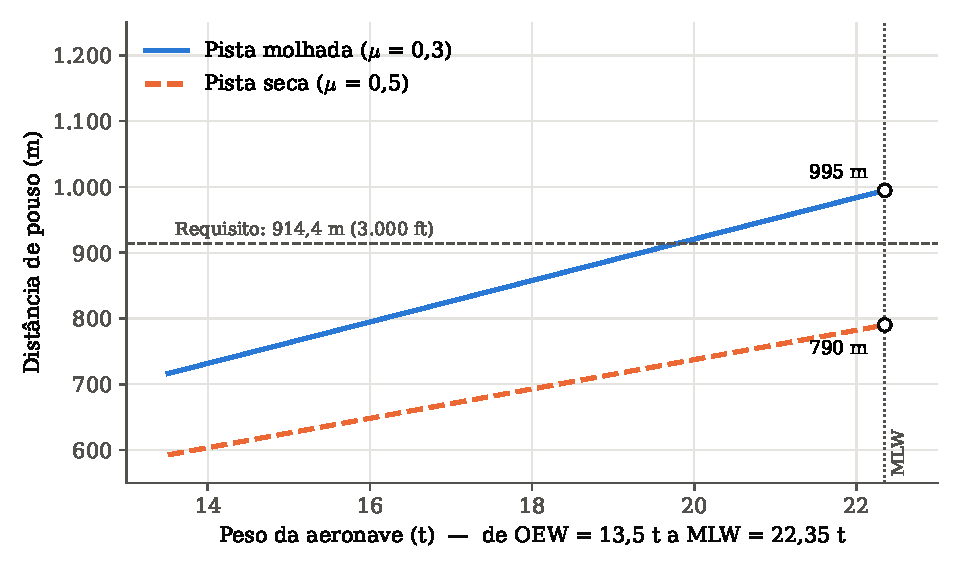
\includegraphics[width=0.7\textwidth]{images/fig7_11_pouso_peso.pdf}
    \caption{Distâncias de Pouso para a aeronave projetada.}
    \label{fig:distancias_pouso}
\end{figure}

Pode-se observar que a aeronave projetada apresentou um bom condicionamento para pistas padrão de pouso em voos regionais de transporte de passageiros/carga.

\section{Voo em Curva}

A avaliação das manobras em curva visa estabelecer o menor raio de giro ($R_{T}$) viável para a aeronave, garantindo não apenas a integridade estrutural, mas também a segurança durante os procedimentos de espera (\textit{holding}) e alinhamento típicos da aviação comercial em áreas de controle terminal. Tratando-se de uma curva coordenada e mantendo a altitude constante, o raio torna-se dependente do quadrado da velocidade aerodinâmica verdadeira ($V_{TAS}$) e da inclinação lateral aplicada ($\phi$), conforme a clássica relação:
\begin{equation}
    R_{T} = \frac{V_{TAS}^{2}}{g \cdot \tan(\phi)}
    \label{eq:raio_curva}
\end{equation}

Estipulou-se uma manobra a nível do mar, utilizando um fator de carga de segurança da ordem de $n = 1,3$. O ângulo de rolamento para curva coordenada \textit{bank angle} requisitado para suportar este esforço aparente obedece à equação geométrica:
\begin{equation}
    \phi = \arccos\left(\frac{1}{n}\right) = \arccos\left(\frac{1}{1,3}\right) \approx 39,71^{\circ}
\end{equation}

Sob a ótica dos requisitos de segurança, a velocidade durante a execução do giro deve apresentar uma folga de margem em relação ao estol, adotando-se o padrão de $1,3 \cdot V_{S0}$. Recorrendo à polar da aeronave em condição \textit{full-flap} ao nível do mar ($42,69 \text{ m/s}$), a velocidade tangencial demandada na trajetória de curva é dada por:
\begin{equation}
    V_{TAS} = 1,3 \times 42,69 \approx 55,5 \text{ m/s}
\end{equation}

Incorporando estas matrizes de dados na formulação central (Equação \ref{eq:raio_curva}), mapeia-se o raio operacional da máquina:
\begin{equation}
    R_{T} = \frac{(55,5)^{2}}{9,81 \cdot \tan(39,71^{\circ})}
\end{equation}
\begin{equation}
    R_{T} \approx 378,11 \text{ m}
\end{equation}


\section{Autonomia e Alcance}

O alcance (\textit{range}) e a autonomia (\textit{endurance}) foram estimados por meio das equações de Bréguet para aeronaves propelidas por hélice. Essas relações são utilizadas como uma aproximação da fase de cruzeiro, considerando voo reto e nivelado e parâmetros propulsivos representativos da condição analisada.

Como o consumo específico adotado é referido à potência no eixo, em $\mathrm{lb/(shp\cdot h)}$, utiliza-se a formulação de Bréguet baseada em potência, e não em tração.

O alcance no trecho de cruzeiro ($R$) é estimado pela Equação \ref{eq:breguet_alcance}:

\begin{equation}
    R = \frac{\eta_{\mathrm{prop}}}{c}
    \frac{C_L}{C_D}
    \ln\left(\frac{W_1}{W_2}\right)
    \label{eq:breguet_alcance}
\end{equation}

De forma análoga, a autonomia no trecho de cruzeiro é estimada pela Equação \ref{eq:breguet_autonomia}:

\begin{equation}
    E =
    \frac{\eta_{\mathrm{prop}}}{c}
    \frac{C_L^{3/2}}{C_D}
    \sqrt{2\rho S}
    \left(
    \frac{1}{\sqrt{W_2}}-
    \frac{1}{\sqrt{W_1}}
    \right)
    \label{eq:breguet_autonomia}
\end{equation}

Nessas equações, $\eta_{\mathrm{prop}}$ representa a eficiência propulsiva da hélice e $c$ o consumo específico de combustível referido à potência no eixo. Os termos $W_1$ e $W_2$ correspondem aos pesos da aeronave no início e no fim do trecho de cruzeiro, respectivamente.

Para a obtenção das curvas, cada altitude foi analisada separadamente, mantendo-se $\rho$ e o peso de referência constantes e variando-se a velocidade verdadeira. Para cada velocidade, o coeficiente de sustentação necessário ao voo nivelado foi calculado por:

\begin{equation}
    C_L = \frac{2W}{\rho V^2 S},
\end{equation}

e o coeficiente de arrasto foi obtido a partir da polar parabólica

\begin{equation}
    C_D = C_{D_0} + K C_L^2.
\end{equation}

Dessa forma, a razão $L/D=C_L/C_D$ varia com a velocidade, mesmo para uma mesma altitude. Assim, as Figuras \ref{fig:alcance_max} e \ref{fig:autonomia_max} representam varreduras de velocidade realizadas a altitude constante.

Com essas relações, foram obtidas as curvas de alcance e autonomia em função da velocidade verdadeira, apresentadas nas Figuras \ref{fig:alcance_max} e \ref{fig:autonomia_max}.

\begin{figure}[H]
    \centering
    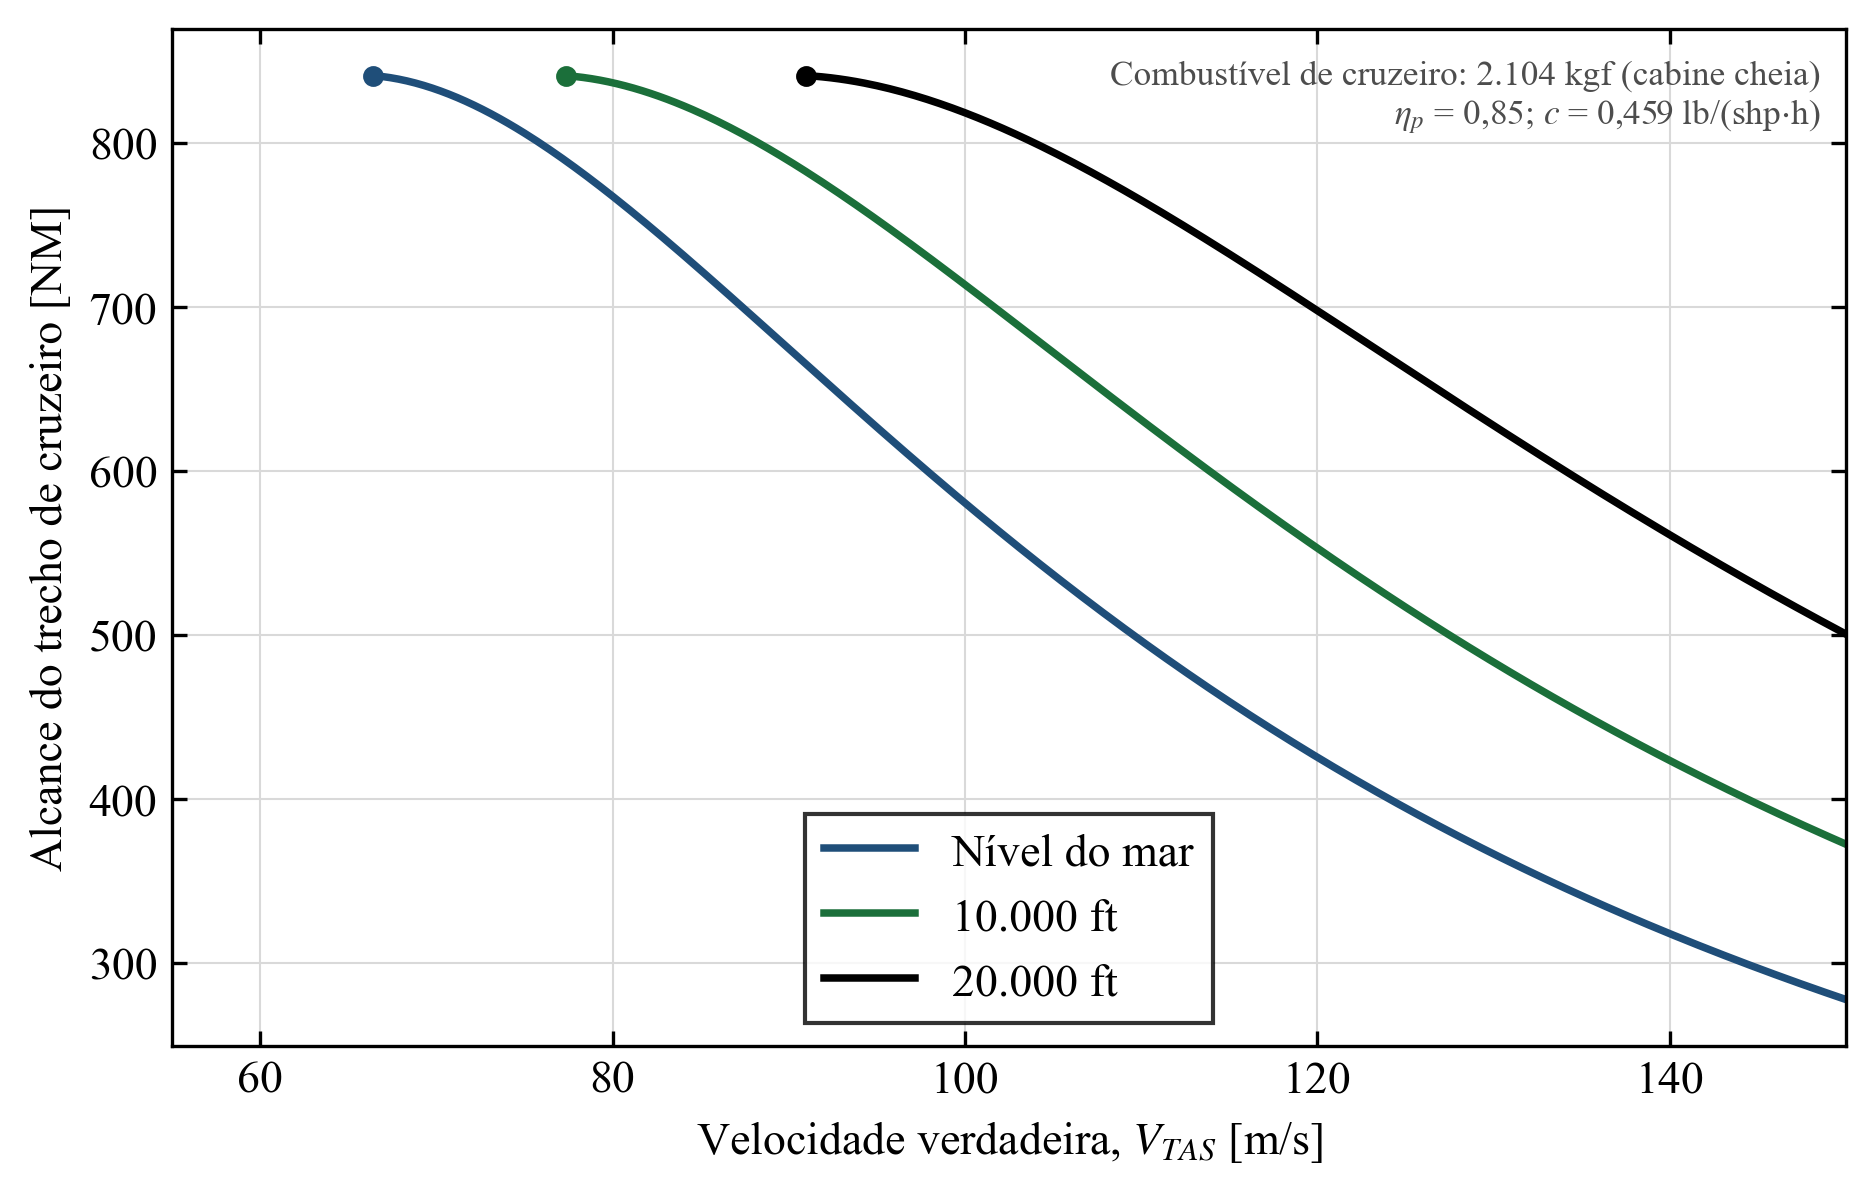
\includegraphics[width=0.8\textwidth]{images/alcance_max.png} 
    \caption{Alcance do trecho de cruzeiro em função da velocidade, com os 2.104~kgf de combustível de cruzeiro da missão com cabine cheia (Tabela~\ref{tab:combustivel_missao}), $\eta_{\mathrm{prop}} = 0{,}85$ e velocidades acima de $1{,}2\,V_S$.}
    \label{fig:alcance_max}
\end{figure}

\begin{figure}[H]
    \centering
    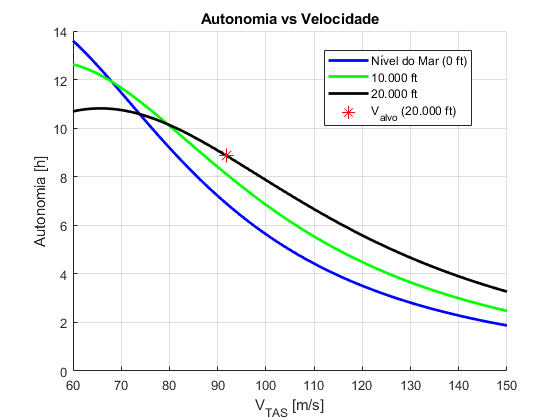
\includegraphics[width=0.8\textwidth]{images/autonomia_max.png}
    \caption{Autonomia do trecho de cruzeiro em função da velocidade, nas mesmas condições da Figura~\ref{fig:alcance_max}.}
    \label{fig:autonomia_max}
\end{figure}

Para uma polar parabólica, considerando peso e altitude constantes durante cada análise e assumindo $\eta_{\mathrm{prop}}$ e $c$ constantes, as velocidades teóricas associadas ao máximo alcance e à máxima autonomia são dadas por:

\begin{equation}
    V_{R_{max}} = \sqrt{\frac{2W}{\rho S}} \sqrt[4]{\frac{K}{C_{D_{0}}}}
\end{equation}
\begin{equation}
    V_{E_{max}} = \sqrt{\frac{2W}{\rho S}} \sqrt[4]{\frac{K}{3C_{D_{0}}}}
\end{equation}

O sumário dos limites estratégicos atingidos por esta configuração, mapeados ao nível do mar e na altitude operacional padrão de cruzeiro, encontra-se elucidado na Tabela \ref{tab:resultados_alcance}.

\begin{table}[H]
    \centering
    \caption{Resultados operacionais para autonomia e alcance máximos.}
    \vspace{0.2cm}
    \small
    \begin{tabular}{lccc}
        \toprule
        \textbf{Parâmetro} & \textbf{\makecell{Nível do Mar \\ (MSL)}} & \textbf{\makecell{Altitude de \\ 10000 ft}} & \textbf{\makecell{Altitude de Cruzeiro \\ (20000 ft)}} \\
        \midrule
        Vel. Máx Autonomia $V_{E_{max}}$ (m/s) & 50,3 & 58,5 & 68,9 \\
        Vel. Máx Alcance $V_{R_{max}}$ (m/s) & 66,2 & 77,0 & 90,7 \\
        \bottomrule
    \end{tabular}
    \label{tab:resultados_alcance}
    \caption*{Calculadas no MTOW, com $C_{D0} \approx 0,040$ e $K \approx 0,032$ ajustados à polar da Tabela 7.11.}
\end{table}

\subsection{Alcance da Missão de Projeto}
\label{sec:alcance_missao}

O alcance da missão de projeto foi calculado com a cabine cheia (64 passageiros com bagagem despachada) e decolagem no MTOW. Nessa condição o combustível a bordo é de 3.088~kgf (Tabela~\ref{tab:cg_pesos}), e não uma fração arbitrária da capacidade dos tanques. Esse combustível foi distribuído entre as fases da missão e as reservas IFR do requisito de alcance (alternativa a 100~NM e 45~minutos de espera, Seção~\ref{section:Requisitos}), com as seguintes hipóteses:

\begin{itemize}
    \item partida, táxi e decolagem com fração de peso de 0,995; descida e pouso com 0,997 cada;
    \item subida até 20.000~ft com o ângulo de $4{,}60^{\circ}$ do diagrama de missão, com o combustível obtido pela energia fornecida, $W\,\Delta h + D\,s$, com eficiência propulsiva de 0,80;
    \item cruzeiro a 20.000~ft pela Equação~\ref{eq:breguet_alcance}, com $c = 0{,}459~\mathrm{lb/(shp\cdot h)}$, $C_L$ constante na condição de máximo alcance limitada a $1{,}3\,V_S$ ($C_L = 0{,}89$, $V \approx 193$~kt TAS, $L/D = 13{,}8$ e $\eta_{\mathrm{prop}} = 0{,}85$, da tabela de eficiência da hélice em cruzeiro) e a polar de cruzeiro do CEA-VLM;
    \item descida em rampa de $3^{\circ}$, que percorre 116~km (Tabela~\ref{tab:fases_missao});
    \item reservas: alternativa a 100~NM em cruzeiro a 10.000~ft e espera de 45~minutos a 1.500~ft na velocidade de potência mínima.
\end{itemize}

\begin{table}[H]
    \centering
    \caption{Distribuição do combustível na missão de projeto (cabine cheia, MTOW).}
    \label{tab:combustivel_missao}
    \begin{tabular}{lcc}
        \toprule
        \textbf{Fase} & \textbf{Combustível [kgf]} & \textbf{Distância [NM]} \\
        \midrule
        Partida, táxi e decolagem & 113 & -- \\
        Subida até 20.000 ft & 246 & 41 \\
        Cruzeiro a 20.000 ft & 2.104 & 821 \\
        Descida e pouso & 121 & 63 \\
        Reserva: alternativa a 100 NM & 248 & -- \\
        Reserva: espera de 45 min & 256 & -- \\
        \midrule
        \textbf{Total} & \textbf{3.088} & \textbf{925} \\
        \bottomrule
    \end{tabular}
\end{table}

O alcance com a cabine cheia é de 925~NM, acima do requisito de 800~NM. Para voar exatamente 800~NM com as mesmas reservas são necessários 2.749~kgf de combustível, de modo que sobram cerca de 340~kgf. A aeronave pousa com cerca de 20.100~kgf, abaixo do MLW de 22.350~kgf. Com o combustível do trecho de cruzeiro voado na velocidade de potência mínima, a autonomia desse trecho é de cerca de 4,7~h (Tabela~\ref{tab:autonomia_alcance_cruzeiro}).

\begin{table}[H]
\centering
\caption{Alcance e autonomia da missão de projeto (cabine cheia, reservas IFR).}
\begin{tabular}{cc}
\hline
Alcance (NM) & Autonomia do trecho de cruzeiro (h) \\
\hline
925 & 4,7 \\
\hline
\end{tabular}
\label{tab:autonomia_alcance_cruzeiro}
\end{table}

\subsection{Diagrama de Carga Paga--Alcance}
\label{sec:carga_paga_alcance}

O diagrama de carga paga--alcance (Figura~\ref{fig:carga_paga_alcance}) mostra as combinações de passageiros, carga e combustível que respeitam o MTOW, o MZFW e a capacidade dos tanques, com o mesmo modelo de missão e as mesmas reservas da Tabela~\ref{tab:combustivel_missao}. Ele é definido pelos quatro pontos da Tabela~\ref{tab:pontos_carga_paga}:

\begin{itemize}
    \item \textbf{A}: carga paga máxima (6.080~kgf), limitada pelo MZFW, sem combustível de missão;
    \item \textbf{B}: carga paga máxima e combustível até o MTOW (3.088~kgf). Entre A e B, a carga paga é limitada pelo MZFW;
    \item \textbf{C}: tanques cheios (4.990~kgf) no MTOW, com a carga paga reduzida para 4.178~kgf. Entre B e C, cada quilograma-força de combustível a mais exige um a menos de carga paga, para não ultrapassar o MTOW;
    \item \textbf{D}: tanques cheios e nenhuma carga paga (voo de translado), decolando com 18.502~kgf.
\end{itemize}

Os pontos B e C são os limites da Tabela~\ref{tab:cg_cargapaga}. Em nenhum ponto o peso de pouso ultrapassa o MLW.

\begin{table}[H]
    \centering
    \caption{Pontos do diagrama de carga paga--alcance.}
    \label{tab:pontos_carga_paga}
    \small
    \begin{tabular}{cccccc}
        \toprule
        \textbf{Ponto} & \textbf{Carga paga} & \textbf{Combustível} & \textbf{Peso de decolagem} & \textbf{Alcance} & \textbf{Limitado por} \\
        \midrule
        A & 6.080 kgf & 0 kgf & 19.592 kgf & 0 NM    & MZFW \\
        B & 6.080 kgf & 3.088 kgf & 22.680 kgf & 925 NM  & MZFW e MTOW \\
        C & 4.178 kgf & 4.990 kgf & 22.680 kgf & 1.767 NM & MTOW e tanques \\
        D & 0 kgf & 4.990 kgf & 18.502 kgf & 2.265 NM & Tanques \\
        \bottomrule
    \end{tabular}
\end{table}

\begin{figure}[H]
    \centering
    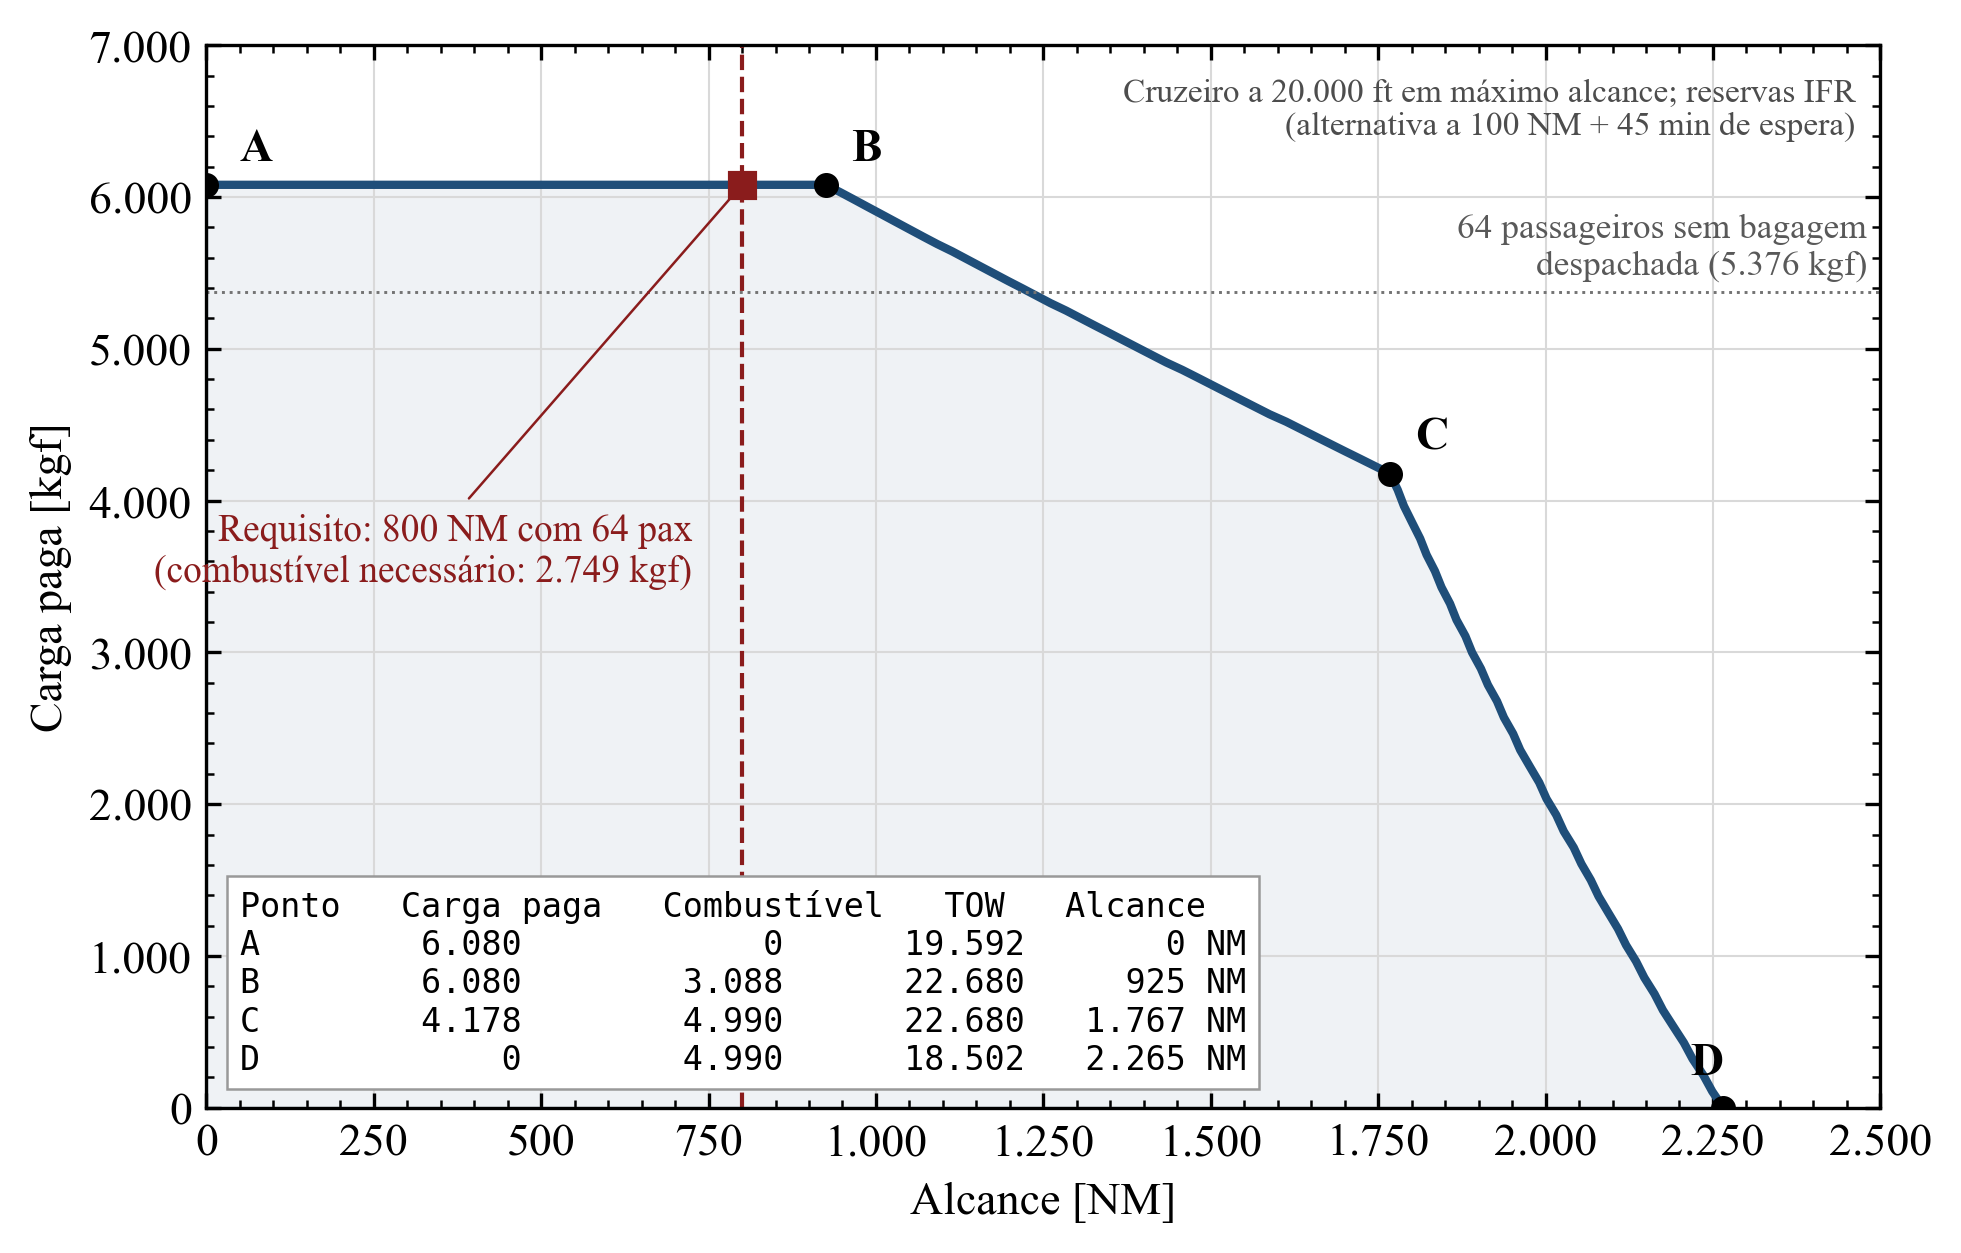
\includegraphics[width=0.95\textwidth]{images/Imagem - desempenho/carga_paga_alcance.png}
    \caption{Diagrama de carga paga--alcance com cruzeiro a 20.000~ft em máximo alcance e reservas IFR (alternativa a 100~NM e 45~min de espera). O quadrado marca o requisito de 800~NM com 64 passageiros.}
    \label{fig:carga_paga_alcance}
\end{figure}


\section{Envelope de Voo}


O envelope de voo é a representação gráfica que delimita a região operacional segura da aeronave em termos de altitude e velocidade verdadeira ($V_{TAS}$). A construção deste diagrama baseia-se na sobreposição dos limites aerodinâmicos (estol) e propulsivos (tração disponível versus necessária).

\subsection{Metodologia}

Para a obtenção do envelope de voo, foi desenvolvido um algoritmo computacional em MATLAB que realiza uma varredura iterativa em altitudes variando do nível do mar até o teto absoluto da aeronave. O procedimento de cálculo para cada altitude $h$ consiste nos seguintes passos:

\begin{enumerate}
    \item \textbf{Cálculo das Propriedades Atmosféricas:} Determinação da densidade do ar ($\rho$) conforme o modelo da Atmosfera Padrão (ISA).
    \item \textbf{Correção da Tração:} A curva de tração disponível ao nível do mar ($T_{SL}$) é corrigida pela razão de densidade ($\sigma = \rho / \rho_0$), assumindo-se um comportamento de motor aspirado:
    \begin{equation}
        T_{disp}(h, V) = T_{SL}(V) \cdot \sigma
    \end{equation}
    \item \textbf{Determinação das Potências:} Cálculo vetorial da Potência Disponível ($P_D = T_{disp} \cdot V$) e da Potência Requerida ($P_R = D \cdot V$) para uma faixa ampla de velocidades.
    \item \textbf{Obtenção dos Limites de Velocidade:} Identificação das interseções entre as curvas de $P_D$ e $P_R$.
\end{enumerate}

\subsection{Definição dos Limites do Envelope}

O envelope é delimitado por duas fronteiras principais:

\textbf{1. Limite Aerodinâmico (Esquerdo):} Definido pela velocidade de estol ($V_S$) na configuração limpa. Esta velocidade aumenta com a altitude devido à redução da densidade do ar, conforme a relação:
\begin{equation}
    V_S = \sqrt{\frac{2 \cdot W}{\rho \cdot S \cdot C_{L_{max}}}}
\end{equation}

\textbf{2. Limite Propulsivo (Direito e Teto):} Definido pela velocidade máxima ($V_{max}$) onde a potência disponível iguala a potência requerida.

Uma consideração crítica realizada no algoritmo é a determinação do limite mínimo de voo em grandes altitudes. Conforme a aeronave sobe, a curva de potência requerida se desloca para cima e para a direita (aumento do arrasto induzido e necessidade de maior $V_{TAS}$), enquanto a potência disponível decresce.

Em altitudes elevadas, a velocidade mínima sustentável pelo motor ($V_{min\_P}$) pode exceder a velocidade de estol aerodinâmico ($V_S$). Portanto, o limite esquerdo do envelope ($V_{esq}$) é definido computacionalmente pela lógica:
\begin{equation}
    V_{esq} = \max(V_S, V_{min\_P})
\end{equation}

Esta consideração explica a curvatura da fronteira esquerda do envelope em altitudes próximas ao teto, onde a aeronave entra no "segundo regime de comando" e a limitação torna-se propulsiva, e não mais puramente aerodinâmica.

\subsection{Resultados do Envelope}

A Figura \ref{fig:envelope_de_voo} apresenta o envelope de voo calculado no MTOW, com a área alar de 74,1~m$^2$ (a versão anterior desta análise usava 54,1~m$^2$, diferente da área alar de 74,1~m$^2$ do projeto). Observa-se que a região operacional se estreita com o ganho de altitude até convergir para um único ponto: o Teto Absoluto. Neste ponto, $V_{min} = V_{max}$, indicando que a aeronave possui apenas uma velocidade possível de voo nivelado e a razão de subida é nula.

\begin{figure}[H]
    \centering
    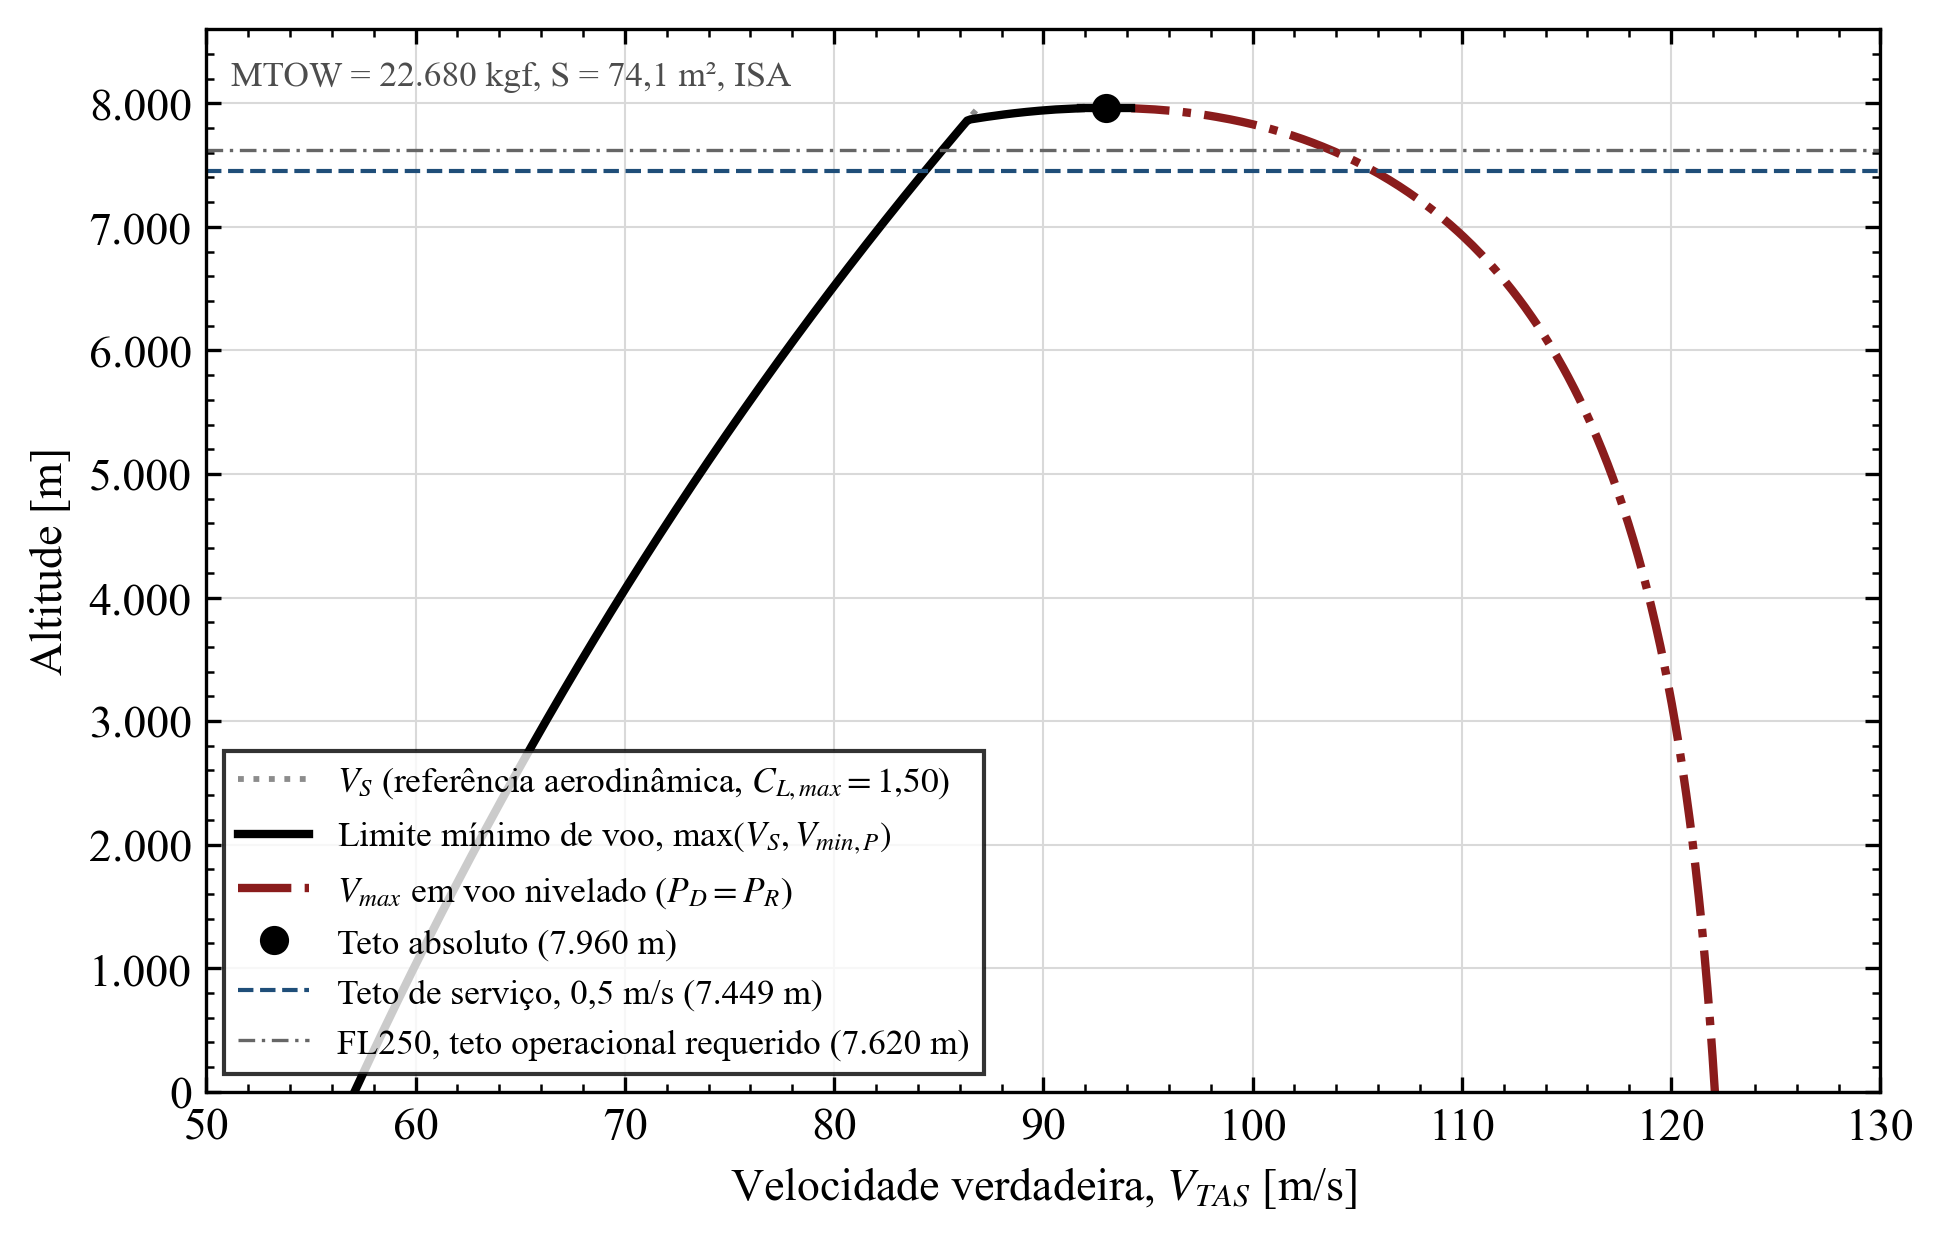
\includegraphics[width=0.9\linewidth]{images/Imagem - desempenho/envelope_voo.png}
    \caption{Envelope de voo no MTOW ($S = 74{,}1$~m$^2$, ISA): limite inferior de estol ou de potência, velocidade máxima em voo nivelado e tetos.}
    \label{fig:envelope_de_voo}
\end{figure}

Com os cálculos obteve-se um teto absoluto de 7.960~m (26.115~ft). A velocidade máxima em voo nivelado é de 122,1~m/s (237~kt) ao nível do mar e de 114,0~m/s (222~kt TAS) a 20.000~ft.

\subsection{Envelope de Operação}
\label{sec:envelope_operacao}

O envelope de operação (Figura~\ref{fig:envelope_operacao}) reúne, em altitude-pressão e velocidade verdadeira, os limites aerodinâmicos e propulsivos do envelope de voo e os limites estruturais e operacionais definidos para a certificação:

\begin{itemize}
    \item velocidade de estol 1~g com flaps recolhidos ($V_{S1}$, $C_{L,max} = 1{,}50$);
    \item velocidade máxima em voo nivelado, limitada pela potência disponível;
    \item velocidade máxima operacional $V_{MO}$, adotada igual a $V_C = 230$~kt EAS, já que o \S 25.1505 do 14 CFR Part 25 não permite $V_{MO}$ maior que $V_C$ (Seção~\ref{sec:cargas_vn});
    \item velocidade de mergulho de projeto $V_D = 288$~kt EAS (\S 25.335(b)), que não pode ser atingida em operação normal;
    \item teto de serviço, teto absoluto e o FL250 do requisito de teto operacional.
\end{itemize}

Abaixo de cerca de 2.000~ft a velocidade máxima em voo nivelado (237~kt EAS ao nível do mar) supera $V_{MO}$, e o limite à direita passa a ser estrutural. Acima disso, o limite à direita é a potência disponível. O teto de serviço de 24.438~ft fica 562~ft abaixo do FL250 requerido, de modo que o teto operacional certificável, no MTOW, fica limitado pelo teto de serviço. A faixa de cruzeiro a 20.000~ft vai de 193~kt TAS, na condição de máximo alcance, a 222~kt TAS, na potência máxima.

\begin{figure}[H]
    \centering
    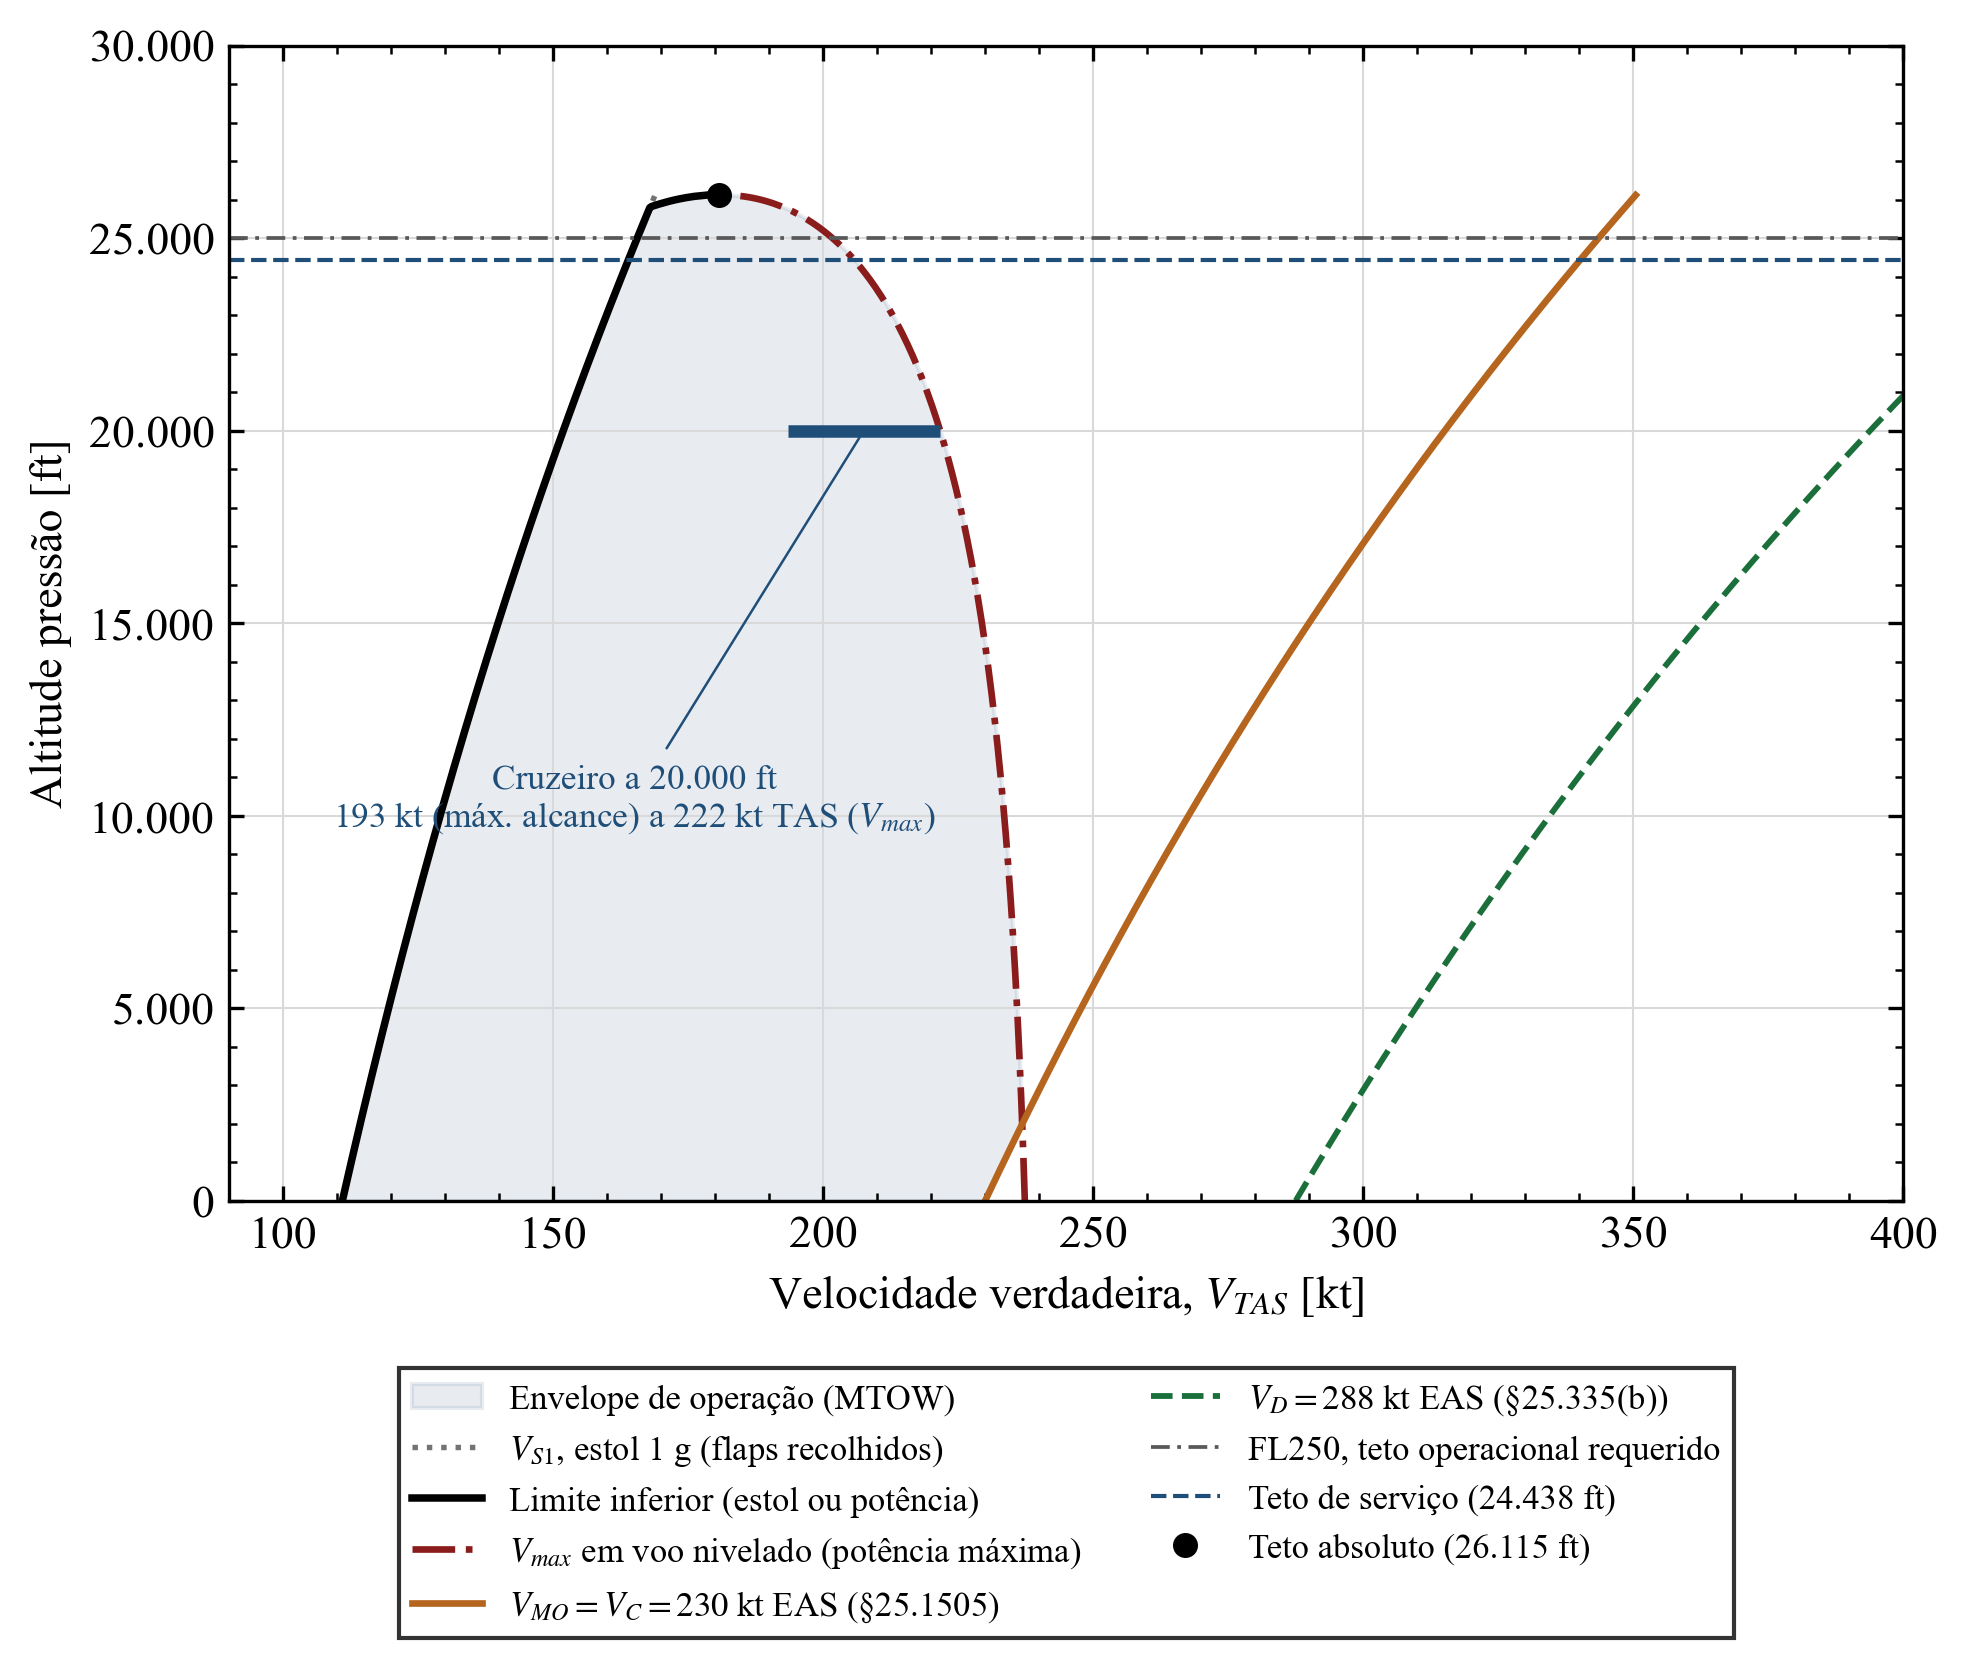
\includegraphics[width=0.95\textwidth]{images/Imagem - desempenho/envelope_operacao.png}
    \caption{Envelope de operação no MTOW: limites de estol, potência, $V_{MO} = V_C$ e $V_D$ (14 CFR Part 25), tetos de serviço e absoluto, FL250 requerido e faixa de cruzeiro a 20.000~ft.}
    \label{fig:envelope_operacao}
\end{figure}



\subsection{Desempenho de Subida}

A capacidade de subida da aeronave é determinada pelo excesso de potência específica (Excess Power). O algoritmo calculou a Razão de Subida ($RC$ - Rate of Climb) para cada velocidade dentro do vetor de análise através da equação:

\begin{equation}
    RC = \frac{P_{disp} - P_{req}}{W}
\end{equation}

Para cada altitude analisada, o código identificou o valor máximo dessa função ($RC_{max}$), que corresponde à melhor taxa de subida possível naquela condição atmosférica.

A Figura \ref{fig:desempenho_subida} ilustra a degradação da razão de subida máxima com o aumento da altitude. O ponto onde a curva intercepta o eixo horizontal (altitude) corresponde ao teto absoluto teórico, onde $RC_{max} = 0$. Para fins operacionais, destaca-se também o Teto de Serviço, definido como a altitude onde a razão de subida cai para 0,5 m/s (aproximadamente 100 ft/min).



\begin{figure}[H]
    \centering
    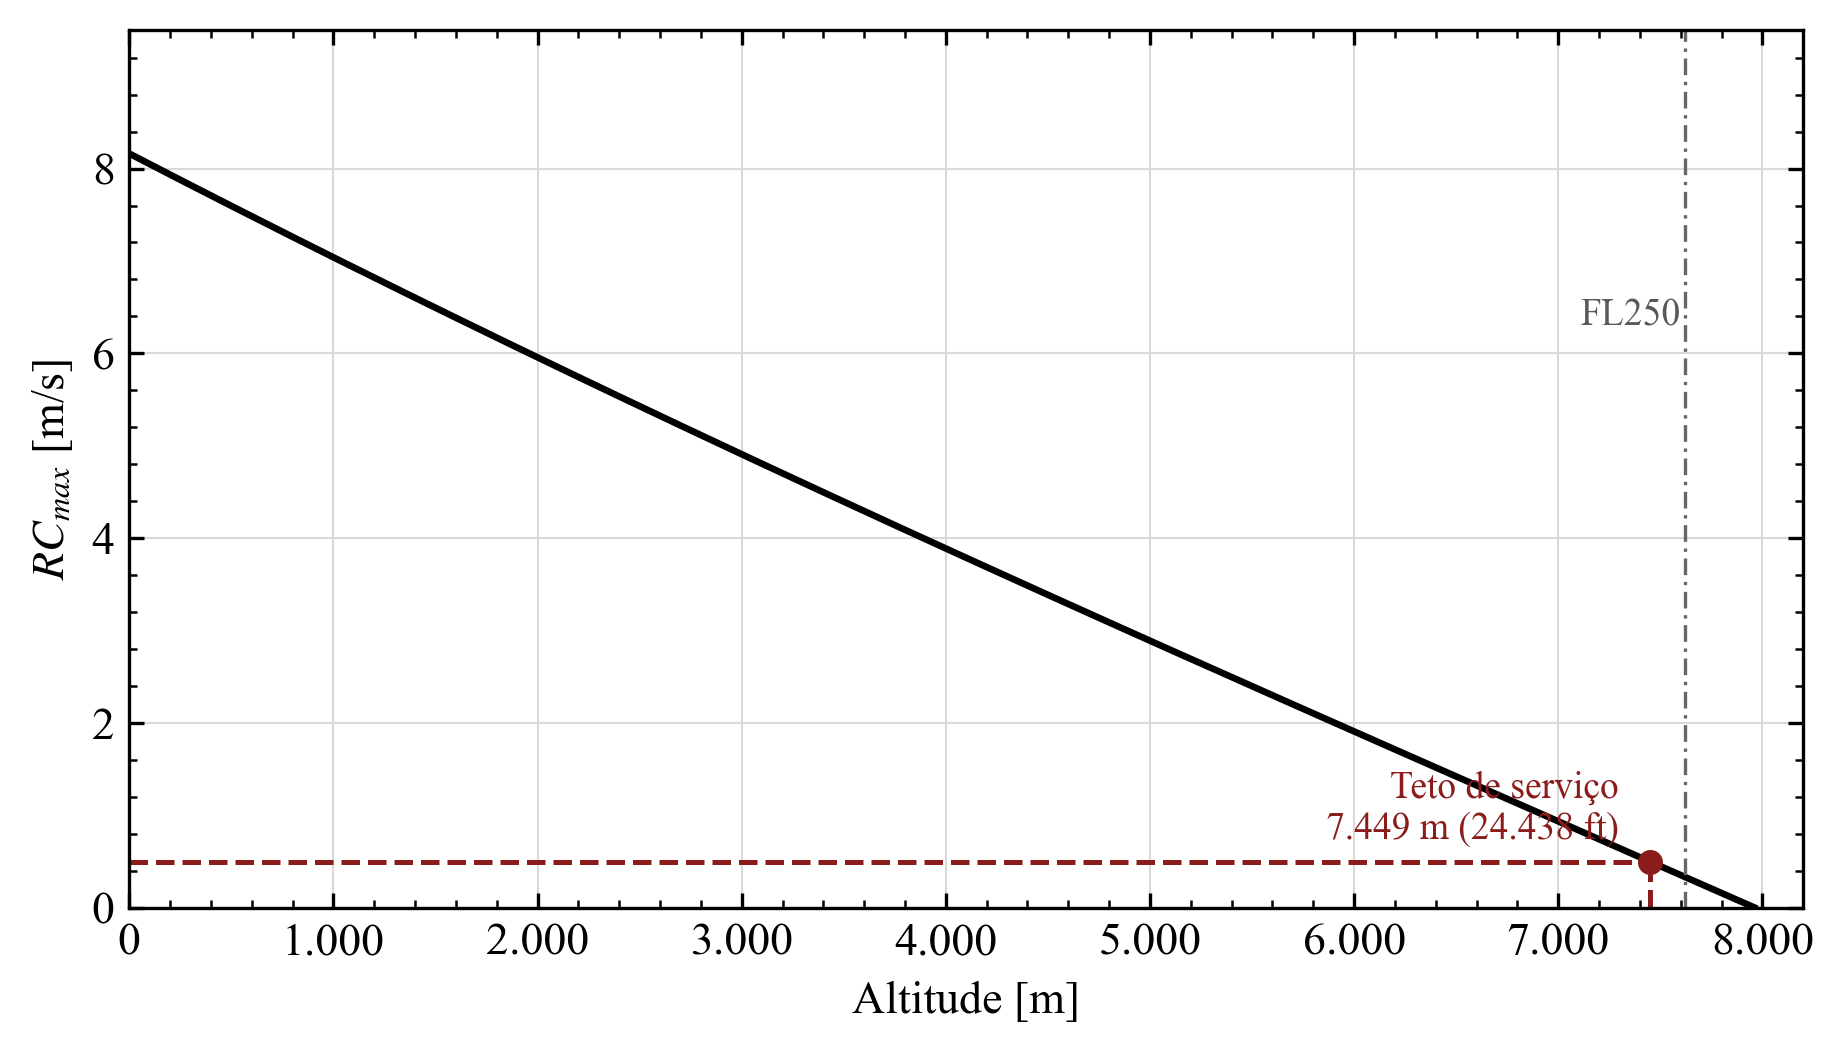
\includegraphics[width=0.9\linewidth]{images/Imagem - desempenho/desempenho_subida.png}
    \caption{Razão de subida máxima em função da altitude, no MTOW ($S = 74{,}1$~m$^2$).}
    \label{fig:desempenho_subida}
\end{figure}


Assim, obteve-se um teto de serviço de 7.449~m (24.438~ft). A 20.000~ft, a razão de subida máxima é de 1,81~m/s (356~ft/min).



\section{Diagrama de Missão}

O Diagrama de Missão representa o perfil de voo calculado para a aeronave em projeto, ilustrando a variação da altitude em função da distância horizontal percorrida desde a decolagem até o pouso completo.

Este perfil foi elaborado considerando as condições de Atmosfera Padrão (ISA), peso máximo de decolagem (MTOW) de 22.680 kgf e operação de pista ao nível do mar. A missão atende a operação baseando-se no alcance máximo estipulado de 800 NM (1.481,6 km), com a etapa de cruzeiro realizada no teto operacional de 20.000 pés.

\subsection{Parâmetros da Missão}

A Tabela \ref{tab:fases_missao} consolida as distâncias horizontais percorridas e as variações de altitude em cada segmento da missão. As distâncias de subida e descida foram projetadas no solo com base no ângulo geométrico de subida calculado ($\gamma \approx 4{,}60^{\circ}$) e numa rampa de aproximação padrão do sistema ILS ($3^{\circ}$).

\begin{table}[H]
    \centering
    \caption{Discriminação das fases da missão típica.}
    \label{tab:fases_missao}
    \vspace{0.2cm}
    \resizebox{\textwidth}{!}{%
    \begin{tabular}{llrrrr}
        \toprule
        \textbf{Fase} & \textbf{Segmento} & \textbf{Distância (m)} & \textbf{Distância (ft)} & \textbf{Alt. Inicial (ft)} & \textbf{Alt. Final (ft)} \\
        \midrule
        \textbf{1. Decolagem} & Corrida no Solo & 907{,}5 & 2.977 & 0 & 0 \\
                              & Transição até Obstáculo & 194{,}1 & 637 & 0 & 35 \\
        \midrule
        
        \textbf{2. Subida}    & \textit{Climb} contínuo & 75.580{,}0 & 247.967 & 35 & 20.000 \\
        \midrule
        
        \textbf{3. Cruzeiro}  & Voo Nivelado & 1.289.992{,}0 & 4.232.257 & 20.000 & 20.000 \\
        \midrule
        
        \textbf{4. Descida}   & Rampa de Planeio & 116.028{,}0 & 380.668 & 20.000 & 50 \\
        \midrule
       
        \textbf{5. Pouso}     & Aproximação e Arredondamento & 329{,}8 & 1.082 & 50 & 0 \\
                              & Corrida de Frenagem & 460{,}2 & 1.510 & 0 & 0 \\
    
        \bottomrule
    \end{tabular}
    }
\end{table}

\subsection{Descrição das Fases}

As características operacionais de cada etapa, ilustradas na Figura \ref{fig:diagrama_missao}, são descritas a seguir:

\begin{enumerate}
    \item \textbf{Decolagem:} A aeronave inicia a missão com uma corrida no solo  de 907,5 m até atingir a velocidade de rotação. Após a decolagem, considera-se uma distância horizontal de 194,1 m para o ganho de altura e ascensão em segurança até a altura do obstáculo padrão de 35 pés (\S25.113). A distância total de decolagem requerida é de aproximadamente 1.102 m.
    
    \item \textbf{Subida (\textit{Climb}):} A partir de 35 pés, a aeronave ascende até a altitude de cruzeiro de 20.000 pés. Sustentada pela potência excedente dos motores acoplados, a aeronave mantém um ângulo de trajetória de voo de $4{,}60^{\circ}$, percorrendo horizontalmente cerca de 75,5 km até atingir o nível de voo no ponto TOC (\textit{Top of Climb}).
    
    \item \textbf{Cruzeiro:} É a fase predominante da missão, onde a aeronave estabiliza em voo reto e nivelado sob regime de potência eficiente. A distância desta etapa é extraída do balanço total da missão, cobrindo quase 1.290 km para garantir o fechamento do alcance estipulado de 800 NM.
    
    \item \textbf{Descida:} Inicia-se no ponto ideal de descida TOD (\textit{Top of Descent}). Assumindo uma rampa de descida padrão de $3^{\circ}$ típica de voos comerciais de passageiros e carga, a aeronave percorre uma distância de solo de aproximadamente 116 km até interceptar a altitude do obstáculo da cabeceira (50 pés).
    
    \item \textbf{Pouso:} Compreende a aproximação aérea final descendo dos 50 pés, o arredondamento de 78 m para redução abrupta da razão de descida e o toque na pista (\textit{Touchdown}). Após o impacto, inicia-se a corrida de frenagem no solo de 460 m. A distância total da fase de pouso situa-se na margem segura de 790 m.
\end{enumerate}

\begin{figure}[H]
    \centering
        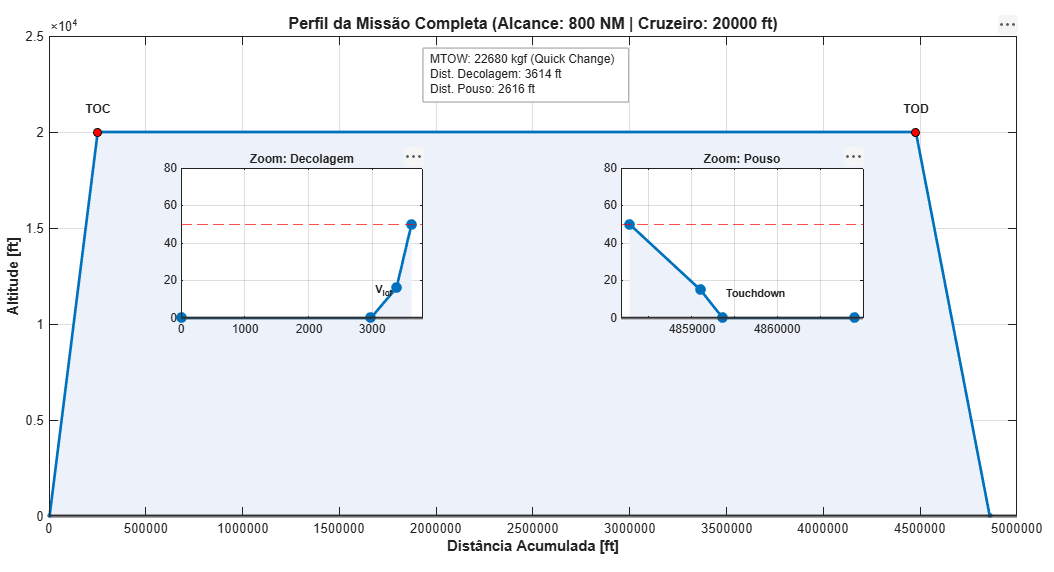
\includegraphics[width=1.0\textwidth]{images//Imagem - desempenho/diagrama de missão.png}
    \caption{Perfil de missão e trajetórias de pista (Altitude vs. Distância Acumulada) para a aeronave proposta.}
    \label{fig:diagrama_missao}
\end{figure}

\newpage
\section{Resumo dos Cálculos de Desempenho da Aeronave}

A tabela \ref{tab:resumo_desempenho} a seguir sumariza a maior parte dos cálculos e estimativas do desempenho da aeronave projetada. É interessante notar que os valores aqui calculados são satisfatoriamente competitivos para o mercado daquele tipo de missão que se pretende realizar com a presente aeronave.


\begin{table}[H]
    \centering
    \caption{Resumo de Desempenho da Aeronave}
    \label{tab:resumo_desempenho}
    \renewcommand{\arraystretch}{1.3} 
    
    % --- INÍCIO DO RESIZEBOX ---
    \resizebox{\textwidth}{!}{%
    \begin{tabular}{@{}llc@{}}
        \toprule
        \textbf{Categoria} & \textbf{Parâmetro} & \textbf{Valor de Projeto} \\
        \midrule
        
        \multirow{3}{*}{\textbf{Pesos e Capacidades}}
        & Peso Máximo de Decolagem (MTOW) & 22.680 kgf (50.000 lb) \\
        & Peso Máximo de Pouso (MLW) & 22.350 kgf (49.273 lb) \\
        & Peso Vazio Operacional (OEW) &
        13.512 kgf (29.789 lb) \\
        \midrule
        
        \multirow{2}{*}{\textbf{Motorização}}
        & Grupo Motopropulsor & 2x Pratt \& Whitney PW127M \\
        & Potência de Decolagem (por motor) & 2.475 shp \\
        \midrule
        
        \multirow{5}{*}{\textbf{Velocidades}}
        & Velocidade de Cruzeiro de Máximo Alcance (20.000 ft) & 193 kt TAS \\
        & Velocidade Máxima em Cruzeiro ($V_{max,cru}$) & 222 kt \\
        & Velocidade Máxima de Decolagem ($V_{max,TO}$) & 193,8 kt \\
        & Velocidade de Estol, flap 40° (MLW) & 82,4 kt \\
        & Razão de Subida Máxima para Cruzeiro ($RC_{max,cru}$) & 1,81 m/s \\
        \midrule
        
        \multirow{3}{*}{\textbf{Operação em Pista (MSL)}}
        & Distância Total de Decolagem & 1.102 m (3.614 ft) \\
        & Distância Física de Pouso & 790 m (2.592 ft) \\
        & Comprimento de Pista Balanceado (BFL) & 1620 m (5.315 ft) \\
        \midrule
        
        \multirow{4}{*}{\textbf{Limites de Missão}}
        & Alcance com Cabine Cheia e Reservas IFR & 925 NM (requisito: 800 NM) \\
        & Autonomia do Trecho de Cruzeiro (cabine cheia) & 4,7 horas \\
        & Teto de Serviço & 24.438 ft (7.449 m) \\
        & Teto Absoluto & 26.115 ft (7.960 m) \\
                
        \bottomrule
    \end{tabular}
    } % --- FIM DO RESIZEBOX ---
    
\end{table}